\documentclass[letterpaper]{article}
\usepackage[margin=1in]{geometry}
\usepackage[utf8]{inputenc}
\usepackage{textcomp}
\usepackage{amssymb}
\usepackage{natbib}
\usepackage{graphicx}
\usepackage{gensymb}
\usepackage{amsthm, amsmath, mathtools}
\usepackage[dvipsnames]{xcolor}
\usepackage{enumerate}
\usepackage{mdframed}
\usepackage[most]{tcolorbox}
\usepackage{csquotes}
% https://tex.stackexchange.com/questions/13506/how-to-continue-the-framed-text-box-on-multiple-pages

\tcbuselibrary{theorems}

\newcommand{\R}{\mathbb{R}}
\newcommand{\Z}{\mathbb{Z}}
\newcommand{\N}{\mathbb{N}}
\newcommand{\Q}{\mathbb{Q}}
\newcommand{\C}{\mathbb{C}}
\newcommand{\code}[1]{\texttt{#1}}
\newcommand{\mdiamond}{$\diamondsuit$}
\newcommand{\PowerSet}{\mathcal{P}}
\newcommand{\Mod}[1]{\ (\mathrm{mod}\ #1)}
\DeclareMathOperator{\lcm}{lcm}

%\newtheorem*{theorem}{Theorem}
%\newtheorem*{definition}{Definition}
%\newtheorem*{corollary}{Corollary}
%\newtheorem*{lemma}{Lemma}
\newtheorem*{proposition}{Proposition}


\newtcbtheorem[number within=section]{theorem}{Theorem}
{colback=green!5,colframe=green!35!black,fonttitle=\bfseries}{th}

\newtcbtheorem[number within=section]{definition}{Definition}
{colback=blue!5,colframe=blue!35!black,fonttitle=\bfseries}{def}

\newtcbtheorem[number within=section]{corollary}{Corollary}
{colback=yellow!5,colframe=yellow!35!black,fonttitle=\bfseries}{cor}

\newtcbtheorem[number within=section]{lemma}{Lemma}
{colback=red!5,colframe=red!35!black,fonttitle=\bfseries}{lem}

\newtcbtheorem[number within=section]{example}{Example}
{colback=white!5,colframe=white!35!black,fonttitle=\bfseries}{def}

\newtcbtheorem[number within=section]{note}{Important Note}{
        enhanced,
        sharp corners,
        attach boxed title to top left={
            xshift=-1mm,
            yshift=-5mm,
            yshifttext=-1mm
        },
        top=1.5em,
        colback=white,
        colframe=black,
        fonttitle=\bfseries,
        boxed title style={
            sharp corners,
            size=small,
            colback=red!75!black,
            colframe=red!75!black,
        } 
    }{impnote}
\usepackage[utf8]{inputenc}
\usepackage[english]{babel}
\usepackage{fancyhdr}
\usepackage[hidelinks]{hyperref}

\pagestyle{fancy}
\fancyhf{}
\rhead{CSE 30}
\chead{June 5th, 2021}
\lhead{Course Notes}
\rfoot{\thepage}

\setlength{\parindent}{0pt}

\begin{document}

\begin{titlepage}
    \begin{center}
        \vspace*{1cm}
            
        \Huge
        \textbf{CSE 30 Notes}
            
        \vspace{0.5cm}
        \LARGE
        Computer Organization and Systems Programming
            
        \vspace{1.5cm}
            
        \vfill
            
        Spring 2021\\
        Taught by Professor Brian Chin
    \end{center}
\end{titlepage}

\pagenumbering{gobble}

\newpage 

\pagenumbering{gobble}
\begingroup
    \renewcommand\contentsname{Table of Contents}
    \tableofcontents
\endgroup

\newpage
\pagenumbering{arabic}

\section{Number Systems}
In this section, we will briefly discuss the different number systems used, with emphasis placed on binary numbers.

\subsection{Common Number Bases}
There are four common number bases:
\begin{center}
    \begin{tabular}{c|c|c|c}
        \textbf{Base} & \textbf{Symbols} & \textbf{Name} & \textbf{Examples} \\ 
        \hline 
        2 & 0, 1 & Binary & 0b101101111 \\ 
        8 & 0-7 & Octal & 0321 \\ 
        10 & 0-9 & Decimal & 1234 \\ 
        16 & 0-9, a-f (10-16) & Hexadecimal & 0xfedba123
    \end{tabular}
\end{center}

There are a few things we should point out. In particular, when written out:
\begin{itemize}
    \item \textbf{Binary} numbers always start with \code{0b}. 
    \item \textbf{Octal} numbers always start with \code{0}.
    \item \textbf{Hexadecimal} numbers always start with \code{0x}. The letters can be uppercase or lowercase.
\end{itemize}
Sometimes, the base will be written as a subscript directly after the number. For example, we can write \code{0b10101} like $10101_{2}$. 

\subsection{Positional Encoding and Significance}
Each place (digit) represents some power of the base. Consider a number with $n$ digits laid out like so\footnote{For example, if we have the number \code{123}, then this number has 3 digits, so $n = 3$. This means that $d_{n - 1} = d_{3 - 1} = d_2 = 1$, $d_{n - 2} = d_{2 - 1} = d_{1} = 2$, and so on.}:
\[d_{n - 1} d_{n - 2} \dots d_3 d_2 d_1 d_0\]
Where $d_i$ is a digit in a specific place. Using a polynomial, we can represent this number like so:
\begin{equation*}
    \begin{aligned}
        \text{Number} &= \sum_{i = 0}^{n - 1} d_i b^i \\ 
            &= d_{n - 1} b^{n - 1} + d_{n - 2} b^{n - 2} + \dots + d_2 b^2 + d_1 b^1 + d_0 b^0
    \end{aligned}
\end{equation*}
Here, $d$ is the digit and $b$ is the base. 

\bigskip 

We call the left-most digit, or the $(n - 1)$th digit, the \emph{most significant digit} since this digit contributes a lot to the number as a whole. We call the right-most digit, or the $0$th place, the \emph{least significant digit} since this digit contributes very little to the number as a whole. For instance, consider the decimal number \code{12345}, which has $n = 5$ digits. We can write this number out using the polynomial representation:
\[\sum_{i = 0}^{5 - 1} a_i b^i = 1 \cdot 10^4 + 2 \cdot 10^3 + 3 \cdot 10^2 + 4 \cdot 10^1 + 5 \cdot 10^0 = 10000 + 2000 + 300 + 40 + 5 = 12345\]\
\begin{itemize}
    \item Here, we know that $1 \cdot 10^4 = 10000$, which contributes the most to the overall number. Thus, 1 is the most significant digit. 
    \item We also know that $5 \cdot 10^0 = 5$ contributes the least to the overall number. Thus, 5 is the least significant digit. 
\end{itemize}

This same exact concept can be applied to numbers of different bases (binary, octal, hexadecimal, and other bases). For instance, if we consider the number \code{0b10101} (which has $n = 5$ digits), we know that\footnote{Here, we have performed binary addition, which will be discussed later on.}:
\[\sum_{i = 0}^{5 - 1} a_i b^i = 1 \cdot 2^4 + 0 \cdot 2^3 + 1 \cdot 2^2 + 0 \cdot 2^1 + 1 \cdot 2^0 = 10000 + 0 + 100 + 0 + 1 = 0b10101\]

\subsection{Converting Between Bases}
Often times, we'll need to convert between different bases. Here, we'll summarize how to do this. 

\subsubsection{Binary and Hexadecimal}
To convert between binary and hexadecimal numbers, we should note that every four-bit sequence (i.e. 4 binary digits) corresponds to one hexadecimal number. The following table gives a better idea of how this works\footnote{Note that this table is basically counting from 0 to 15 in both binary and hexadecimal. In this sense, you should not have to memorize this table.}:

\begin{center}
    \begin{tabular}{c|c}
        \textbf{Binary} & \textbf{Hexadecimal} \\ 
        \hline 
        \code{0000} & \code{0} \\ 
        \code{0001} & \code{1} \\ 
        \code{0010} & \code{2} \\ 
        \code{0011} & \code{3} \\ 
        \code{0100} & \code{4} \\ 
        \code{0101} & \code{5} \\ 
        \code{0110} & \code{6} \\ 
        \code{0111} & \code{7} \\ 
        \code{1000} & \code{8} \\ 
        \code{1001} & \code{9} \\ 
        \code{1010} & \code{A} (10) \\ 
        \code{1011} & \code{B} (11) \\ 
        \code{1100} & \code{C} (12) \\ 
        \code{1101} & \code{D} (13) \\ 
        \code{1110} & \code{E} (14) \\ 
        \code{1111} & \code{F} (15)
    \end{tabular}
\end{center}

The conversion between binary and hexadecimal works like so:
\begin{itemize}
    \item To convert from binary to hexadecimal, begin by dividing up the bits into chunks of four, from \underline{right to left}. If the left-most chunk does not have 4 bits, you can pad that chunk with leading zeroes until you have 4 bits. Then, you can make use of the above table. 
    
    \bigskip 

    For instance, to convert \code{0xb491} to binary, note that:
    \begin{verbatim}
        b       4       9       1
        1011    0100    1001    0001    ->      0b1011010010010001
    \end{verbatim}

    \item To convert from hexadecimal to binary, simply translate each individual hexadecimal digit to its corresponding binary number. 
    
    \bigskip

    For instance, to convert \code{0b1111011001} to hexadecimal:
    \begin{verbatim}
        0b1111011001 
        -> 11 1101 1001         (Break into chunks of four)
        -> 0011 1101 1001       (Pad the left-most chunk if needed)
        -> 3    d    9          (Convert to hexadecimal digits)
        -> 0x3d9                (Combine)
    \end{verbatim}
\end{itemize}

\subsubsection{Binary and Octal}
The idea is exactly the same as when converting between binary and hexadecimal. The only difference is that we are dealing with every \underline{three}-bit sequence (i.e. 3 binary digits) as opposed to a four-bit sequence. In other words, every three-bit sequence corresponds to one octal number. The following table gives a better idea of how this works\footnote{Same idea as with the previous footnote. The only difference is that we're counting from 0 to 7 in both binary and octal.}:
\begin{center}
    \begin{tabular}{c|c}
        \textbf{Binary} & \textbf{Hexadecimal} \\ 
        \hline 
        \code{000} & \code{0} \\ 
        \code{001} & \code{1} \\ 
        \code{010} & \code{2} \\ 
        \code{011} & \code{3} \\ 
        \code{100} & \code{4} \\ 
        \code{101} & \code{5} \\ 
        \code{110} & \code{6} \\ 
        \code{111} & \code{7}
    \end{tabular}
\end{center}

Aside from this difference, the process of converting between binary and octal is basically the same as with binary and hexadecimal.  


\subsubsection{Hexadecimal and Octal}
To convert between hexadecimal and octal, we can simply take the immediate step of finding the binary representation of a number and \emph{then} converting that binary representation to the other base.

\bigskip 

For instance, suppose we have the octal number \code{0763} (or $763_8$). The binary representation of this number is:
\begin{verbatim}
    111 110 011
\end{verbatim} 
Regrouping these bits gives us\footnote{Note that we padded three zeroes in the left-most chunk.}:
\begin{verbatim}
    0001 1111 0011
\end{verbatim}
And then converting this to hexadecimal gives us \code{0x1f3}.


\subsubsection{Converting to Decimal}
Converting to decimal is very straightforward. Consider a number with $n$ digits that is in base $b$. Then, the most significant digit is the $(n - 1)$th digit (the left-most digit) and the least significant digit is the 0th digit (the right-most digit). For every digit $d_i$ (where $i$ is the location of the digit relative to the least significant digit), we have:
\begin{equation*}
    \begin{aligned}
        \text{Number} &= \sum_{i = 0}^{n - 1} d_i b^i \\ 
            &= d_{n - 1} b^{n - 1} + d_{n - 2} b^{n - 2} + \dots + d_2 b^2 + d_1 b^1 + d_0 b^0
    \end{aligned}
\end{equation*}

You can use this same formula to find the decimal form of any given base. 

\bigskip 

For instance, if we have the hexadecimal number \code{0xb491}, we know that the base is 16 and the most significant digit is $b$, which is located at position 3 ($n = 4$ and $4 - 1 = 3$). Then:
\[11 \cdot 16^3 + 4 \cdot 16^2 + 9 \cdot 16^1 + 1 \cdot 16^0 = 46225\]
So, the hexadecimal number \code{0xb491} is equivalent to \code{46225} in decimal. 


\subsubsection{Converting from Decimal}
To do this, we make use of an algorithm.
\begin{itemize}
    \item Given \code{number} and base \code{b}.
    \item Start with the least-significant digit (\code{n = 0}). 
    \item Repeat until \code{number == 0}:
    \begin{itemize}
        \item Divide \code{number} by \code{b} to produce a quotient and remainder. 
        \item Place the remainder in the $b^n$ position. 
        \item Let \code{number = quotient}. 
        \item Increment \code{n} by one. 
    \end{itemize}
\end{itemize}

For instance, let's suppose we have $72_{10}$ and we wanted to convert this number to base 7. Using this algorithm, we have:
\begin{itemize}
    \item $n = 0$ with \code{number = 72}: $\frac{72}{7} = 10$ with remainder \textbf{2} (least-significant digit).
    \item $n = 1$ with \code{number = 10}: $\frac{10}{7} = 1$ with remainder \textbf{3}. 
    \item $n = 2$ with \code{number = 1}: $\frac{1}{7} = 0$ with remainder \textbf{1} (most-significant digit).
\end{itemize}
So, it follows that $71_{10} = 132_{7}$. 

\subsection{Signed vs. Unsigned Binary Integers}
An \emph{unsigned} integer is simply an integer that is strictly non-negative. A \emph{signed} integer is simply an integer that can be negative, positive, or zero.

\subsubsection{Signed Magnitude and One's Complement}
Signed magnitude simply treats the high-order bit as a sign bit. That is, instead of including the most significant bit (sign bit) as part of the number, we only use the most-significant bit to determine if the number is positive (\code{0xxx...}) or negative (\code{1xxx...}). 

\bigskip 

Computing a decimal value for an $n$-bit signed magnitude sequence is simple: simply calculate the value of the digits $d_0$ through $d_{n - 2}$ using the method discussed in the first page and then change the sign of this number based on the most significant bit. 

\bigskip 

To negate the value, we simply take the \emph{one's complement}, or simply flip the bits such that all \code{0}s become \code{1}s and all \code{1}s becomes \code{0}s. 

\bigskip 

However, this suffers from one major drawback: there are two representations of zero. For instance, for 4-bit binary, \code{0b1000} represents \code{-0} while \code{0b0000} represents \code{+0}. 

\subsubsection{Two's Complement}
We can solve the issue presented by one's complement by using the two's complement encoding. Here, the most significant bit (the sign bit) will determine the sign of the number while also being included in the computation of the number itself. 

\bigskip 

If the sign bit is \code{0}, then we can compute the number like so:
\[d_{n - 2} \cdot 2^{n - 2} + \dots + d_2 \cdot 2^2 + d_1 \cdot 2^1 + d_0 \cdot 2^0\]
If the sign bit is \code{1}, then we must also include the sign bit in the computation, which can be done like so:
\[- d_{n - 1} \cdot 2^{n - 1} + d_{n - 2} \cdot 2^{n - 2} + \dots + d_2 \cdot 2^2 + d_1 \cdot 2^1 + d_0 \cdot 2^0\]
It follows that the range is simply $-2^{n - 1} \leq x \leq 2^{n - 1} - 1$. 

\bigskip 

To negate the value, we simply take the \emph{one's complement} like usual, but then also add one to the resulting value. In other words:
\begin{itemize}
    \item Flip all bits. 
    \item Add one to result.
\end{itemize}

For instance, to negate \code{0111} (\code{7}), flip all bits (\code{1000}) and then add one (\code{1001}). Thus, the negation of \code{0111} is \code{1001} (\code{-7}).

\subsection{Binary Arithmetic}
It should be noted that the paper-and-pencil method that we learned can easily be applied to binary arithmetic. Thus, we will not cover this in great detail.

\subsubsection{Binary Addition}
This is exactly the same as doing regular addition, except that you are restricted to \code{0} and \code{1} instead of what we're used to with the decimal system. 

\subsubsection{Binary Subtraction}
Same deal. However, we should note that two's complement can be used to make things easier. In particular, it should be noted that:
\[A - B = A + (-B)\]
So, we can easily use two's complement to negate $B$, thus allowing us to add $A$ and $-B$ without having to deal with actual subtraction.

\subsubsection{Binary Multiplication and Division}
Same deal. It should be noted that, with binary division, the fractional part will always be truncated. 

\subsubsection{Multiplying and Dividing by Powers of 2}
Consider the following table.
\begin{center}
    \begin{tabular}{c|c|c|c|c|c|c}
            & $a_5 \cdot 2^5$ & $a_4 \cdot 2^4$ & $a_3 \cdot 2^3$ & $a_2 \cdot 2^2$ & $a_1 \cdot 2^1$ & $a_0 \cdot 2^0$ \\
            \hline
            10 &  & & 1 & 0 & 1 & 0 \\
            20 & & 1 & 0 & 1 & 0 & 0 \\
            40 & 1 & 0 & 1 & 0 & 0 & 0 \\
            5  & & & & 1 & 0 & 1
    \end{tabular}
\end{center}
To multiply a number by a power of two, we can simply shift the bits one to the left. For division, we can shift the bits one to the right. In C or C++, this can be represented like so:
\begin{verbatim}
    int a = 10;
    
    int b = a << 1; // 10 * 2^1 = 20
    int c = a >> 1; // 10 / 2^1 = 5 

    int d = a << 2; // 10 * 2^2 = 40
    int e = a >> 2; // 10 / 2^2 = 2
\end{verbatim}

\subsection{Overflow}
When dealing with a fixed number of bits, we need to be aware of limitations. In particular, if we have a fixed number of bits, we cannot store some numbers.

\bigskip 

Detecting overflow is relatively straightforward. 
\begin{itemize}
    \item Add the two numbers. 
    \item If the sign bits are different, we cannot have overflow. In other words, $A + (-B)$ or $(-A) + B$ will not produce an overflow. 
    \item Two positive numbers must sum to a positive number. 
    \item Two negative numbers must sum to a negative number. 
\end{itemize}

For instance, \code{1000 - 0001 = 1000 + 1111} will result in an overflow, as will \code{0110 + 0111}. 

\subsection{Fixed Point Numbers}
This is relatively straightforward. Basically, a fixed point number is a number with a \emph{fixed} number of digits after the decimal point. 

\bigskip 

We can only represent a fixed point number of the form $\frac{x}{2^k}$ for $x, k \in \Z$. Otherwise, we will have repeating bits. 

\bigskip 

We can express fixed point numbers in polynomial form, similar to how we did it with integers, like so:
\[d_{n - 1} b^{n - 1} + d_{n - 2} b^{n - 2} + \dots + d_1 b^1 + d_0 b^0 + d_{-1} b^{-1} + d_{-2} b^{-2} + \dots\]

For instance, \code{10/4 = 2.5} can be represented by the binary number $10.1$ (you would have to do long division to get this result). 

\subsection{Floating Point Numbers}
We use floating point numbers to express numbers that cannot be expressed using fixed point numbers. 

\subsubsection{Representation}
Generally speaking, we can represent floating point numbers in one of two ways:
\begin{itemize}
    \item Numerically:
    \[(-1)^S M \cdot 2^E\]
    \begin{itemize}
        \item $S$ represents the sign bit. This tells you if the number is negative (\code{1}) or positive (\code{0}).
        \item $M$ represents the mantissa. This is the fractional part of the number (after normalizing). 
        \item $E$ represents the exponent. 
    \end{itemize}

    \item Encoding: 
    \begin{center}
        \begin{tabular}{|c|c|c|}
            \hline 
            \code{s} & \code{exp} \qquad\qquad & \code{frac} \qquad\qquad\qquad\qquad\qquad \\  
            \hline 
        \end{tabular}
    \end{center}

    \begin{itemize}
        \item The \code{s} field is the sign bit. 
        \item The \code{exp} field encodes $E$, but is not equal to $E$.
        \begin{itemize}
            \item We introduce a concept known as a biased exponent. The formula is:
            \[\textbf{exp} = E + \textbf{bias}\]
        \end{itemize}
        \item The \code{frac} field encodes $M$, but is not equal to $M$.
    \end{itemize}
\end{itemize}

\subsubsection{Converting Decimal to Floating Point}
To convert from decimal to floating point, we do the following:
\begin{enumerate}[(1)]
    \item Convert the integer and fraction separately. 
    \begin{itemize}
        \item Convert the integer to a decimal using the algorithm mentioned in page 4. 
        \item For the fractional part, multiply by 2 and use the digit to the left of the decimal as the binary digit. 
    \end{itemize}
    \item Express this number as a binary fixed point.
    \item Normalize. Here, we define a normalized number to be one with a leading \underline{non-zero} digit.  
\end{enumerate}

\subsubsection{Converting Floating Point to Decimal}
To convert from floating point to decimal, we do the following:
\begin{enumerate}[(1)]
    \item Decompose the bits so that you can easily tell what the sign field, exponent field, and mantissa are. 
    \begin{itemize}
        \item Since you are given the exponent field, convert this to the actual exponent by using the formula:
        \[\textbf{exp} = E + \textbf{bias}\]
    \end{itemize}
    
    \item Write out the number in binary scientific notation form:
    \[1.\text{mmmm} \cdot 2^E\]
    Where \code{mmmm} is the mantissa field. 

    \item Expand out the number that you found in the previous step. Then, convert it to decimal. Be sure to account for the sign bit. 
\end{enumerate}

\subsubsection{Examples}
For instance, let's suppose we have a 9-bit floating point format, with an exponent bias of 7 and an exponent field width of 4 bits. Furthermore, let's suppose we are given \code{+0.3125} and want to convert this to its equivalent hexadecimal floating point value. 
\begin{enumerate}[(1)]
    \item We want to convert the integer and fraction separately. 
    \begin{itemize}
        \item The integer value is \code{0}, which is \code{0} in binary. We do not need to do anything with this. 
        \item The fractional value is \code{0.3125}. To convert this to binary:
        \begin{itemize}
            \item $0.3125 \cdot 2 = \mathbf{0}.625$
            \item $0.625 \cdot 2 = \mathbf{1}.25$
            \item $0.25 \cdot 2 = \mathbf{0}.50$
            \item $0.50 \cdot 2 = \mathbf{1}.00$
        \end{itemize}
        So, we have \code{.0101} as our decimal\footnote{When compared to how you would use the algorithm, this is the main difference. In the main algorithm, after we found the digits, we went from bottom-to-top (132 instead of 231 in the example). Here, we're going from top-to-bottom (0101 instead of 1010)}.  
    \end{itemize}
    \item Our binary fixed point is \code{0 + 0.0101 = 0.0101}. 
    \item Normalizing this, we have $1.01 \cdot 2^{-2}$ = $1.0100 \cdot 2^{-2}$. 
    \begin{itemize}
        \item Since the bias is 7, we know that \code{exp = E + bias = -2 + 7 = 5}. In binary, this is \code{0101}. 
        \item The mantissa (\code{frac}) is \code{0100} (we omit the leading \code{1}). 
        \item The sign is \code{0} (the given number is positive).
    \end{itemize}
    \item Encoding this, we have:
    \begin{center}
        \begin{tabular}{c|c|c}
            \code{s} & \code{exp} & \code{frac} \\ 
            \hline 
            \code{0} & \code{0101} & \code{0100}
        \end{tabular}
    \end{center}
    So, our final binary representation is\footnote{Here, we padded the 0s to the left of the sign bit}:
    \begin{verbatim}
        0000 0101 0100
    \end{verbatim}
    And thus, our hexadecimal representation is:
    \begin{verbatim}
        0x054
    \end{verbatim}
\end{enumerate}

For instance, let's suppose we have a 10-bit floating point format, with an exponent bias of 7 and an exponent field of 4 bits rather than 3. What is \code{0x33C} in decimal? 

\begin{enumerate}[(1)]
    \item We want to begin by converting \code{0x33C} to binary. This is simply:
    \begin{verbatim}
        11 0011 1100
    \end{verbatim}
    Decomposing this, we know that:
    \begin{itemize}
        \item \code{1} is the sign bit. This means that the number is negative. 
        \item \code{1001} is the exponent field. We know that $\textbf{exp} = 1001_2 = 9_{10}$. Since the bias is 7, we know that the exponent is:
        \[\textbf{exp} = 9 = E + 7 \iff E = 2\]
        So, the exponent is 2. 
        \item \code{11100} is the mantissa. 
    \end{itemize}
    \item Now, we want to write this number out into scientific notation form. This would look like:
    \[1.11100 \cdot 2^2 = 111.1\]
    \item Converting this to decimal, we have:
    \[2^2 + 2^1 + 2^0 + 2^{-1} = 7.5\]
    Since the sign bit was \code{1}, this number is negative. So, our final answer is:
    \[-7.5\]
\end{enumerate}

\subsubsection{The Denormal Case}
A denormal number is one where the exponent field is all zeroes. \underline{There is no implied leading one.} Despite the exponent field being all zeroes, you can assume that the exponent $E$ will be the lowest possible $E$ (in other words, an exponent field containing all zeroes is the same as the lowest possible exponent field). 


% ================================================%
%                NEW SECTION                      %
% ================================================%7
\newpage 

\section{The \textbf{C} Programming Language}
In this section, we will briefly discuss the C programming language. Heavier emphasis will be placed on pointers, memory management, strings, \code{struct}s, and more. 


\subsection{Basic Data Types}
C has several basic data types.
\begin{itemize}
    \item \code{int}.
    \item \code{char}.
    \item \code{float}.
    \item \code{short}.
    \item \code{long}.
\end{itemize}
By default, these are signed. For example, the following line of code defines a \emph{signed} integer:
\begin{verbatim}
    int x = -5;
\end{verbatim}
If you want the unsigned type, simply prefix the type with \code{unsigned}. For example:
\begin{verbatim}
    unsigned long y = 2;
\end{verbatim}

\subsection{Basic Data Object in Memory}
Consider the following code:
\begin{verbatim}
    int num; 
    num = 20;
\end{verbatim}
Here, we define a variable \code{num} with value \code{20}, which is \code{4} bytes. This will be located in a particular memory address, which will be assigned by the compiler.

\bigskip 

Every variable generally has the following attributes:
\begin{itemize}
    \item The name/identifier - \emph{how will you refer to this variable?}
    \item The value - \emph{What is the value of this variable? In other words, what value is this variable holding?}
    \item The address - \emph{Where in memory is this value located?}
    \item The size - \emph{What is the size of this value? Or, rather, what's the maximum size that this variable can hold?}
    \item The data type - \emph{What is the variable is supposed to be?}
    \item The lifetime - \emph{How long is this variable supposed to last?}
    \item The scope - \emph{Where was this variable defined?}
\end{itemize}

\subsection{Strings}
C does not have a dedicated variable type for strings. Instead, we can think of strings as an \textbf{array of characters} with a null character\footnote{A null character, also known as the null-terminating character, marks the \emph{end} of a string.} at the end. The null character is simply a backslash followed by a zero: \verb"\0".

\bigskip 

Let's consider the string \code{Hello}:
\begin{center}
    \begin{tabular}{c|c|c|c|c|c|c}
        \textbf{Index} & \code{0} & \code{1} & \code{2} & \code{3} & \code{4} & \code{5} \\ 
        \hline 
        \code{char} & \code{'H'} & \code{'e'} & \code{'l'} & \code{'l'} & \code{'o'} & \verb"\0"
    \end{tabular}
\end{center}
We should note the following:
\begin{itemize}
    \item A valid string must have a null character at the end. If it doesn't have a null character, it's not a valid string. 
    \item You must allocate one extra byte in an array for the null character. 
    \item Strings do not always have a newline, so don't depend on a newline being right before the null-terminating character.
    \item Strings are \emph{not} objects. They have no additional embedded information, like string length or methods.
    \item If you must calculate the length of a string, use the C string library \code{strlen} function to calculate the string length. In this case, the null character is not counted.\footnote{Keep in mind that \code{strlen} is $O(n)$ because it must scan the entire string. Thus, if you need the length of the string at a later point, you should save the value.}
\end{itemize}
Consider the string declarations:
\begin{verbatim}
    char mess1[] = "Hello World";
    char mess2[] = {'H', 'e', 'l', 'l', 'o', ' ', 'w', 'o', 'r', 'l', 'd', '\0'};
    char mess3[] = {'H', 'e', 'l', 'l', 'o', ' ', 'w', 'o', 'r', 'l', 'd'};
\end{verbatim}
\code{mess1} is an array that has enough space to hold the contents of the string and the null character (here, an implict null character is added at the end). Thus, \code{mess1} is a valid string. \code{mess2} is exactly the same as \code{mess1}, but more explicit. In memory, \code{mess1} or \code{mess2} would be stored like so\footnote{The byte addresses will be determined by the compiler. These are simply examples.}:
\begin{center}
    \begin{tabular}{c|c}
        \textbf{Value} & \textbf{Byte Address} \\ 
        \hline
        \dots    & \dots      \\
        00110011 & 0x0100000d \\ 
        01000101 & 0x0100000c \\ 
        00000000 (\verb"\0") & 0x0100000b \\ 
        `d'      & 0x0100000a \\ 
        `l'      & 0x01000009 \\ 
        `r'      & 0x01000008 \\ 
        `o'      & 0x01000007 \\ 
        `w'      & 0x01000006 \\ 
        ` '      & 0x01000005 \\ 
        `o'      & 0x01000004 \\ 
        `l'      & 0x01000003 \\ 
        `l'      & 0x01000002 \\ 
        `e'      & 0x01000001 \\ 
        `H'      & 0x01000000
    \end{tabular}
\end{center}

\bigskip 

On the other hand, \code{mess3} is an invalid string since there is not a null-terminating charaacter at the end.

\subsection{Pointers}
A pointer is a variable that contains the address of a variable. In other words, a pointer stores a reference to something. A pointee is the thing that the pointer points to. The address of a variable is simply a number that indicates where the data is stored in memory (we say that this address represents the place in memory where the data lives). 

\bigskip 

A pointer can only point to one type and can represent a basic or derived type such as an \code{int}, \code{char}, a \code{struct}, another pointer, and more. 

\subsubsection{Pointer Declaration}
To declare a pointer, simply put a star (\code{*}) directly before the name of the variable or directly after the data type. For example, the following are all valid\footnote{In my opinion, declaring a pointer as \code{int* x;} (as opposed to \code{int *x;}) makes it more clear what \code{x} is.}:
\begin{verbatim}
    int *x; 
    int* x;
\end{verbatim}
Here, \code{x} is a pointer to an integer. \code{x} is \underline{not} an integer.

\bigskip 

When we declare a pointer like what we did above, we note that \code{x} doesn't actually point to anything yet. We can either:
\begin{itemize}
    \item Make it point to something that already exists. 
    \item Or, allocate room in memory for something new that it will point to. 
\end{itemize}

\subsubsection{Addresses}
To get the address of a variable, simply put an ampersand (\code{\&}) before the name of a variable. For example:
\begin{verbatim}
    int y = 3;
    int* x = &y; 
\end{verbatim}
Here, \code{\&y} gives you the address of \code{y}.\footnote{\code{\&y} is \textbf{not} an address. \code{\&y} gives you the address to \code{y}.}

\subsubsection{Dereference/Indirection Operator}
We can use \code{*} to declare a pointer. We can also use \code{*} to \emph{dereference} a pointer. When we dereference a pointer, we are \emph{retriving} the value from the memory address that is pointed by the pointer. 

\bigskip 

To dereference a pointer, we simply put the \code{*} \emph{before} the pointer variable name. For instance:
\begin{verbatim}
    int x = 10;         // Declare variable "x" that holds value "10"
    int* y = &x;        // Declare int pointer "y" that holds address to x
    int z = *y;         // Declare "z" to be the value "y" is pointing to (dereferencing)
    printf("%i\n", x);  // Prints: 10
    printf("%p\n", y);  // Prints: 0x7ffdd1cd2578 (some memory address)
    printf("%i\n", z);  // Prints: 10
    *y = 5;             // Set the value at address 0x7ffdd1cd2578 to "5"
    printf("%i\n", x);  // Prints: 5
    printf("%p\n", y);  // Prints: 0x7ffdd1cd2578 (same memory address)
    printf("%i", z);    // Prints: 10
\end{verbatim}
As noted in the example, we can also use the dereference operator to:
\begin{itemize}
    \item Change the value located at whatever address the pointer has to a different value.
    \item Set a new variable with the value located at whatever address the pointer is pointing to. 
\end{itemize}

\subsection{Arrays and Pointer Arithmetic}
In C, an array is simply a contiguous (adjacent) region of memory. 

\bigskip 

Declaring an array is as simple as:
\begin{verbatim}
    int arr[5];                   // Declare int array of size 5. If no initial values
                                  // are given, you must explicitly state the size.
    int arr[] = {1, 2, 3, 4, 5};  // Declare int array of size 5 (implicitly) with 
                                  // initial values.
    int arr[5] = {1, 2, 3, 4, 5}; // Declare int array of size 5 (explicitly) with 
                                  // initial values.
    int arr[5] = {1, 2, 3};       // Declare int array of size 5 (explicitly) with 
                                  // some initial values.
\end{verbatim}

A pointer can \emph{point} to an array. In fact, when we define an array, we are given the pointer to the first element. For instance:
\begin{verbatim}
    int arr[3];                 // "arr" is a pointer to the first element in this array.
\end{verbatim}

So, we say that \code{arr} is a pointer to the first element. Then:
\begin{itemize}
    \item \code{arr[0]} is the same as \code{*arr}
    \item \code{arr[2]} is the same as \code{*(arr + 2)}
\end{itemize}

What we did in the second bullet point is known as \emph{pointer arithmetic}. Here's a more concrete example that showcases pointer arithmetic:
\begin{verbatim}
    // Declare an array of 10 int elements.
    // Suppose the first element was located at address 100.
    int array[10];
    // Iterate through every element. 
    // Set every element to its index.
    for (int i = 0; i < 10; i++) {
        // The following two lines are equivalent. 
        *(array + i) = i;
        array[i] = i;
    }
    // Define a pointer to array.
    // ptr is now pointing to the first element (array[0])
    int* ptr = array; 
    // Increment pointer. Now, ptr is pointing to the second element.
    ptr++;
    // Set the second element to 100. Same as: array[1] = 100;
    *ptr = 100; 
    // Decrement pointer. Now, ptr is pointing to the first element.
    ptr--; 
    // Set the first element to 50. Same as: array[0] = 50;
    *ptr = 50; 
\end{verbatim}
A few notes to consider:
\begin{itemize}
    \item \code{*(array + 1)} is \emph{not} the same as \code{*array + 1}. The former is equivalent to \code{array[1]} while the latter is equivalent to \code{array[0] + 1}. 
    \item When doing pointer arithmetic, C will automatically handle the byte size. For instance, when you do \code{*(array + 1)} where \code{array} is an \code{int} array, C will know to add 4 to the pointer (since an \code{int} has 4 bytes).  
\end{itemize}

\subsubsection{Legality of Pointer Operators}
The following are some common pointer arithmetic operators, along with whether said operators are legal. 

\begin{center}
    \begin{tabular}{|c|c|}
        \hline 
        \textbf{Operator} & \textbf{Legal?} \\
        \hline 
        \code{++}, \code{--}, \code{[]}, \code{==}, \code{!=} & Yes \\ 
        Pointers + Integer & Yes \\ 
        Pointer - Integer & Yes \\ 
        Integer - Pointer & No (See 1) \\ 
        Pointer - Pointer & Yes (See 2) \\ 
        Pointer + Pointer & No (See 3) \\ 
        Pointer $\times$ Pointer & No (See 4) \\ 
        \hline
    \end{tabular}
\end{center}
\begin{enumerate}[(1)]
    \item You would have to negate the pointers; pointers are always positive. 
    \item This returns an integer representing the \emph{distance} in elements between pointers.
    \item This is not guaranteed to be an address. 
    \item This is simply repeated addition.
\end{enumerate}

\subsection{Functions}
When we think of a C function, we think of a function that looks something like this:
\begin{verbatim}
    void foo(int x, int y) {
        int tmp; 
        tmp = x;
        x = y;
        y = tmp;
    }
\end{verbatim}
We note a few things.
\begin{itemize}
    \item Parameters are always passed by value.
    \item A function will always have a return type, a name, parameter list, and an implementation.
\end{itemize}

\subsubsection{Header vs. Implementation Files}
When writing a C function, you want to put the function header, or function declaration, in a \code{.h} file (the header file). You put the actual function implementation in the \code{.c} file. For example:
\begin{verbatim}
    // Function headers (.h file). 
    void foo(int x, int y);
    void bar(int, char);

    // Implementation (.c file).
    void foo(int x, int y) {
        int z = x + y;
    }

    void bar(int x, char z) {
        int y = z + x;
    }
\end{verbatim}

\subsubsection{Mimic Pass-by-Reference}
We can use pointers to mimic pass-by-reference. For instance, the \code{swap} function swaps \code{x} and \code{y}:
\begin{verbatim}
    void swap(int* x, int* y) {
        int temp; 
        temp = *x; 
        *x = *y; 
        *y = temp;
    }
\end{verbatim}
To use this function, we pass the addresses of the two variables we want to swap. For example:
\begin{verbatim}
    int x = 5;
    int y = 10;
    swap(&x, &y); 
    // x is 10, y is 5. 
\end{verbatim}
This is still pass-by-value, but we are passing the address instead of the actual value. Thus, it might be more accurate to call this \emph{pass-by-pointer}.

\subsection{Types of Memory}
There are two main types of memory that we are concerned with:
\begin{itemize}
    \item Local variables (and parameters) go on the \emph{stack}.
    \item Dynamically allocated memory goes on the \emph{heap}.
\end{itemize}

\subsection{Allocating Memory at Runtime}
We can allocate memory using \code{malloc}, \code{realloc}, or \code{calloc}. These will go on the \emph{heap}. 

\subsubsection{Allocate Memory: \code{malloc}}
We can allocate memory using \code{malloc}. \code{malloc} has the following function declaration:
\begin{verbatim}
    // malloc initializes the allocate memory with garbage values.
    // - The first argument is the amount of memory to allocate, in bytes. 
    void* malloc(size_t size);
\end{verbatim}
Here, \code{void*} is the return type. \code{void*} is a pointer to anything (so you can cast this pointer to anything). If this is \code{NULL}, then an error occurred. Otherwise, this returns the \emph{base address} of the allocated heap memory. 

\bigskip 

From the \code{man} page:
\begin{displayquote}
    The \code{malloc()} function allocates \underline{\code{size}} bytes and returns a pointer to the allocated memory. The memory is not initialized.  If size is 0, then \code{malloc()} returns either \code{NULL}, or a unique pointer value that can later be successfully passed to \code{free()}.
\end{displayquote}

\subsubsection{Allocate Memory and Zero Out: \code{calloc}}
We can also allocate memory using \code{calloc}\footnote{\code{calloc(5, sizeof(type))} is approximately equivalent to \code{malloc(5 * sizeof(type))}, but the former zeroes out all blocks while the latter keeps the garbage values.}:
\begin{verbatim}
    // calloc initializes the allocated memory with 0 value.
    // - The first argument is the number of blocks to be allocated.
    // - The second argument is the size of each block.   
    void* calloc(size_t nmemb, size_t memsize);
\end{verbatim}

From the \code{man} page:
\begin{displayquote}
    The \code{calloc()} function allocates memory for an array of \underline{\code{nmemb}} elements of \underline{\code{size}} bytes each and returns a pointer to the allocated memory. The memory is set to zero. If \underline{\code{nmemb}} or \underline{\code{size}} is 0, then \code{calloc()} returns either \code{NULL}, or a unique pointer value that can later be successfully passed to \code{free()}.
\end{displayquote}

\subsubsection{Reallocate Memory: \code{realloc}}
If we need to, we can resize a block of memory using the \code{realloc} function:
\begin{verbatim}
    // realloc resizes the memory block pointed to by ptr that 
    // was previously allocated with a call to malloc or calloc. 
    // - The first argument is the pointer to the memory block that 
    //   you want to reallocate. 
    // - The second argument is the new size for the memory block, 
    //   in bytes. If this is zero and ptr points to an existing 
    //   block of memory, then this will deallocate ptr.  
    void* realloc(void* ptr, size_t size);  
\end{verbatim}

From the \code{man} page:
\begin{displayquote}
    The \code{realloc()} function changes the size of the memory block pointed to by \underline{\code{ptr}} to \underline{\code{size}} bytes. The contents will be unchanged in the range from the start of the region up to the minimum of the old and new sizes. If the new \underline{\code{size}} is larger than the old size, the added memory will not be initialized. If \underline{\code{ptr}} is \code{NULL}, then the call is equivalent to \code{malloc(size)}, for all values of \underline{\code{size}}; if \underline{\code{size}} is equal to zero, and \underline{\code{ptr}} is not \code{NULL}, then the call is equivalent to \code{free(ptr)}. Unless \underline{\code{ptr}} is \code{NULL}, it must have been returned by an earlier call to \code{malloc()}, \code{calloc()} or \code{realloc()}. If the area pointed to was moved, a \code{free(ptr)} is done.
\end{displayquote}

\subsubsection{Free Dynamically Allocated Memory: \code{free}}
Of course, when you allocate memory, you must free it (or else it's a memory leak). For this, there's a \code{free} function. \code{free} has the following function declaration:
\begin{verbatim}
    void free(void* ptr);
\end{verbatim}

From the \code{man} page:
\begin{displayquote}
    The \code{free()} function frees the memory space pointed to by \underline{\code{ptr}}, which must have been returned by a previous call to \code{malloc()}, \code{calloc()} or \code{realloc()}. Otherwise, or if \code{free(ptr)} has already been called before, undefined behavior occurs. If \underline{\code{ptr}} is NULL, no operation is performed.
\end{displayquote}

\subsubsection{Basic Example}
Consider the following code:
\begin{verbatim}
    // Allocate an int.
    int* num = malloc(sizeof(int));
    // Free that int.
    free(num); 
    // Allocate an int array of size 10.
    int* arr = malloc(sizeof(int) * 10);
    arr[5] = 10;
    // Free that array.
    free(arr);
\end{verbatim}
All we did was allocate some memory, free it, and then allocate more memory. Simple as that.

\subsection{Structures}
A structure, or \code{struct}, is a data structure composed of simple types. It's simple to classes in Java and C++, but there are no methods or inheritance. 

\subsubsection{General Syntax}
The general syntax for a \code{struct} declaration is:
\begin{verbatim}
    struct struct_name {
        type member1;
        // ... 
        type memberN
    };
\end{verbatim}

\subsubsection{Using an Alias: \code{typedef}}
We can also define an \emph{alias} for the \code{struct}. The syntax for this is as follows:
\begin{verbatim}
    typedef struct struct_name {
        type member1;
        // ... 
        type memberN
    } struct_alias; 
\end{verbatim}
We can also define an alias like so:
\begin{verbatim}
    typedef struct struct_name struct_alias; 
    struct struct_name {
        type member1;
        // ... 
        type memberN
    };
\end{verbatim}

\subsubsection{Defining a Structure}
The following three declarations are equal.
\begin{itemize}
    \item The normal way. 
    \begin{verbatim}
        struct Point {
            int x_coord;
            int y_coord;
        };

        struct Point point; 
    \end{verbatim}

    \item Using an alias.
    \begin{verbatim}
        struct Point {
            int x_coord; 
            int y_coord;
        } p_t;

        p_t point;
    \end{verbatim}
    
    \item The alternative alias. 
    \begin{verbatim}
        typedef struct Point p_t;
        struct Point {
            int x_coord; 
            int y_coord;
        };

        p_t point; 
    \end{verbatim}
\end{itemize}

\subsubsection{Allocating Memory for a Structure}
Suppose we have the above \code{Point} struct. Then, allocating memory is as simple as:
\begin{verbatim}
    // Using the full name.
    struct Point* pt = malloc(sizeof(Point));
    // Using type alias 
    p_t* pt = malloc(sizeof(p_t)); 
\end{verbatim}
The compiler will determine the size of the given \code{struct}. 

\subsubsection{Accessing Members of a Structure}
Suppose we wanted to access the \code{x\_coord} member. There are two ways.
\begin{itemize}
    \item If you are given the structure itself, use the \code{.} (dot) operator. For example:
    \begin{verbatim}
        struct Point pt; 
        pt.x_coord = 5;
        pt.y_coord = 3;
        int sum = pt.x_coord + pt.y_coord;
    \end{verbatim}

    \item If you are given a pointer to the structure, use the \code{->} (arrow) operator. For example:
    \begin{verbatim}
        struct Point* pt = malloc(sizeof(Point));
        pt->x_coord = 5;
        pt->y_coord = 3;
        int sum = pt->x_coord + pt->y_coord;
    \end{verbatim}
    It should be noted that the following two lines are equivalent:
    \begin{verbatim}
        pt->x_coord = 5;
        (*pt).x_coord = 5;
    \end{verbatim}
\end{itemize}

\subsection{Dangling Pointers vs. Memory Leaks}
Here, we will briefly discuss the difference between a dangling pointer and a memory leak, as well as common examples of such. 

\subsubsection{Dangling Pointers}
A \textbf{dangling pointer} is a pointer that points to a memory location that no longer exists. In other words, it's when you free an area of memory but still hvae a pointer to the freed memory. 

\bigskip 

Here are two common examples of dangling pointers. 
\begin{enumerate}
    \item Returning a local address from a function.
    \begin{verbatim}
        char* function() {
            // Note that this is a local declaration! 
            char str[10];
            strcpy(str, "Hello!");
            return str;
        }

        int main() {
            char* hello_string = function(); 
            // Returned pointer points to "str" which has gone out of scope.
            // This is a dangling pointer because "str" no longer exists in 
            // this scope. 
        }
    \end{verbatim}
    
    \item Accessing a memory location that has already been freed. 
    \begin{verbatim}
        int* c = malloc(sizeof(int)); 
        free(c);
        *c = 3;
        // Another example of a dangling pointer because, here, we are writing 
        // to a freed location. In other words, this memory location no longer 
        // exists. 
    \end{verbatim}
\end{enumerate}

\subsubsection{Memory Leaks}
A memory leak is memory in heap that can no longer be accessed. In other words, it's when you lose the pointer but still have the memory allocated. 

\bigskip 

Here are two common examples of memory leaks. 
\begin{enumerate}
    \item Allocating memory but not keeping a pointer to it. 
    \begin{verbatim}
        void function() {
            int* int_array = malloc(5 * sizeof(int));
        }

        // After "function" is done executing, int_array will still be initialized
        // but there won't be a pointer to it. 
    \end{verbatim}

    \item Allocating memory but overwriting it. 
    \begin{verbatim}
        int main() {
            int* array1 = malloc(10 * sizeof(int)); 
            int* array2 = malloc(10 * sizeof(int)); 
            array1 = array2; 
        }
        
        // Here, we created two integer arrays. But, we assigned "array2" to 
        // "array1." Now, we lost all references to the original contents of 
        // "array1," which is a memory leak. 
    \end{verbatim}
\end{enumerate}

% ================================================%
%                NEW SECTION                      %
% ================================================%
\newpage 

\section{32-Bit ARM Assembly (Part I)}
In this section, we will discuss ARM assembly instructions.

\subsection{Arithmetic Instructions}
We begin by talking about arithmetic instructions.

\subsubsection{Format}
Generally speaking, we can write an instruction using the format:
\begin{verbatim}
    opcode  DESTINATION, OPERAND1, OPERAND2
\end{verbatim}
Where \code{opcode} is the instruction by name, \code{DESTINATION} is always the left-most register (right after the opcode), \code{OPERAND1} is the first operand, and \code{OPERAND2} is the second operand. 

\bigskip 

So, for example, suppose we have the following assembly instruction:
\begin{verbatim}
    add     r3, r2, r1
\end{verbatim}
The destination register is \code{r3}; this is where the result goes. Assuming that \code{r3} corresponds to \code{c}, \code{r2} corresponds to \code{b}, and \code{r1} corresponds to \code{a}, this assembly code is equivalent to the C code:
\begin{verbatim}
    c = b + a;
\end{verbatim}
We can also introduce \emph{immediates} (which are otherwise known as \emph{constants}). These are prefixed with a pound symbol (\code{\#}) and will always be the \textbf{last} operand. That is:
\begin{verbatim}
    add     r3, r2, #5    // Valid. 
    add     r3, #5, r2    // Invalid.
\end{verbatim}
In the first line above, we are using the constant \code{5} (notice how it is prefixed by a pound symbol). In C, assuming \code{r3} corresponds to variable \code{c} and \code{r2} corresponds to variable \code{b}, this corresponds to:
\begin{verbatim}
    c = b + 5; 
\end{verbatim}

We can also use binary and hexadecimal numbers in immediates. For example:
\begin{verbatim}
    add     r3, r2, #0xf
\end{verbatim}

\subsubsection{Addition and Subtraction of Integers}
To add two integers, we use the following instruction:
\begin{verbatim}
    add     DESTINATION, OPERAND1, OPERAND2
\end{verbatim}
For example, let's suppose that the C variable \code{c} corresponds to register \code{r3}, \code{b} corresponds to register \code{r2}, and \code{a} corresponds to register \code{r1}. Then, the following C code can be translated to its assembly counterpart:
\begin{verbatim}
    c = b + a;
    add     r3, r2, r1 

    c = a + b;
    add     r3, r1, r2 

    a = b + c; 
    add     r1, r2, r3

    a = a + a;
    add     r1, r1, r1 

    a = b + 2;
    add     r1, r2, #2
\end{verbatim}
To subtract two integers, we use the following instruction: 
\begin{verbatim}
    sub     DESTINATION, OPERAND1, OPERAND2
\end{verbatim}
Using the same example as above, the following C code can be translated to its assembly counterpart:
\begin{verbatim}
    c = b - a;
    sub     r3, r2, r1 

    c = a - b;
    sub     r3, r1, r2 

    a = b - c; 
    sub     r1, r2, r3
    
    a = a - a;
    sub     r1, r1, r1 

    a = b - 2;
    sub     r1, r2, #2
\end{verbatim}
We should note that, if we need to translate some C code which involves the use of orders of operations (for example, the problem \code{f = (g + h) - (i + j)}), we will need to make use of an intermediate temporary register. The general strategy is that we should prioritize operations that have higher precedence (for example, for the example problem, we would make a temporary register for \code{i + j} or \code{g + h} and then subtract the two registers that we used to get the final result). 

\subsubsection{Multiplication of Integers}
To multiply two integers, we use the following instruction: 
\begin{verbatim}
    mul     DESTINATION, OPERAND1, OPERAND2
\end{verbatim}
For example, let's suppose that the C variable \code{c} corresponds to register \code{r3}, \code{b} corresponds to register \code{r2}, and \code{a} corresponds to register \code{r1}. Then, the following C code can be translated to its assembly counterpart:
\begin{verbatim}
    a = b * c; 
    mul     r1, r2, r3

    a = b * 5;
    mul     r1, r2, #5 

    b = b * c;
    mul     r2, r2, r3
\end{verbatim}

\subsubsection{Logical/Bitwise Operators}
There are four basic logical operators: 
\begin{itemize}
    \item \code{AND}
    \item \code{OR}
    \item \code{XOR}
    \item \code{BIC} (Bit Clear)
\end{itemize}
A truth table can better demonstrate how each operation works. 
\begin{center}
    \begin{tabular}{c|c|c|c|c}
        \code{A B} & \code{A AND B} & \code{A OR B} & \code{A XOR B} & \code{A BIC B} \\ 
        \hline 
        \code{0 0} & \code{0} & \code{0} & \code{0} & \code{0} \\ 
        \code{0 1} & \code{0} & \code{1} & \code{1} & \code{0} \\ 
        \code{1 0} & \code{0} & \code{1} & \code{1} & \code{1} \\ 
        \code{1 1} & \code{1} & \code{1} & \code{0} & \code{0}
    \end{tabular}
\end{center}
Just like with addition and subtraction, the format for these instructions is exactly the same. So, here are some direct translations: 
\begin{center}
    \begin{tabular}{c|c|c}
        \textbf{Operator} & \textbf{Example (ARM)} & \textbf{Equivalent To (C)} \\ 
        \hline
        Bitwise \code{AND} & \code{and r0, r1, r2} & \code{r0 = r1 \& r2} \\ 
        Bitwise \code{OR} & \code{orr r3, r4, r5} & \code{r3 = r4 | r5} \\ 
        Bitwise \code{XOR} & \code{eor r0, r1, r2} & \code{r0 = r1 \string^ r2} \\
        Bitwise Clear \code{BIC} & \code{bic r3, r4, r5} & \code{r3 = r4 \& (!r5)} 
    \end{tabular}
\end{center}
Some remarks:
\begin{itemize}
    \item Notice how the \code{XOR} operation is actually denoted as \code{EOR} in assembly! 
    \item We can use these bitwise operators (especially \code{AND}) to create a bitmask.
\end{itemize}

\subsubsection{Shift Instructions}
Assume ARM registers \code{r0}, \code{r1} are associated with C variables \code{a} and \code{b}, respectively. Then:
\begin{center}
    \begin{tabular}{c|c|c}
        \textbf{Operator} & \textbf{Example (ARM)} & \textbf{Equivalent To (C)} \\ 
        \hline
        \code{<<} & \code{lsl r0,r1,\#4} & \code{a = b << 4} \\ 
        \code{>>} (Zero Extend) & \code{lsr r0, r1, \#8} & (Maybe) \code{a = b >> 8} \\ 
        \code{>>} (Sign Extend) & \code{asr r0, r1, \#7} & (Maybe) \code{a = b >> 7} 
    \end{tabular}
\end{center}
The difference between \code{ASR} and \code{LSR} are as follows:
\begin{itemize}
    \item \code{LSR} is \textbf{l}ogical \textbf{s}hift \textbf{r}ight. It will shift and the top bits become 0. This is equivalent to dividing an unsigned integer by a power of 2.
    \item \code{ASR} is \textbf{a}rithmetical \textbf{s}hift \textbf{r}ight. It will shift the number, taking into account if the number is positive or negative, essentially preserving the highest bit. This has the effect of dividing a signed integer by a power of 2.
\end{itemize}
A visual diagram\footnote{Note that we are using 8-bits for illustration purposes.} is shown below (courtesy of Professor Chin from his review video):
\begin{center}
    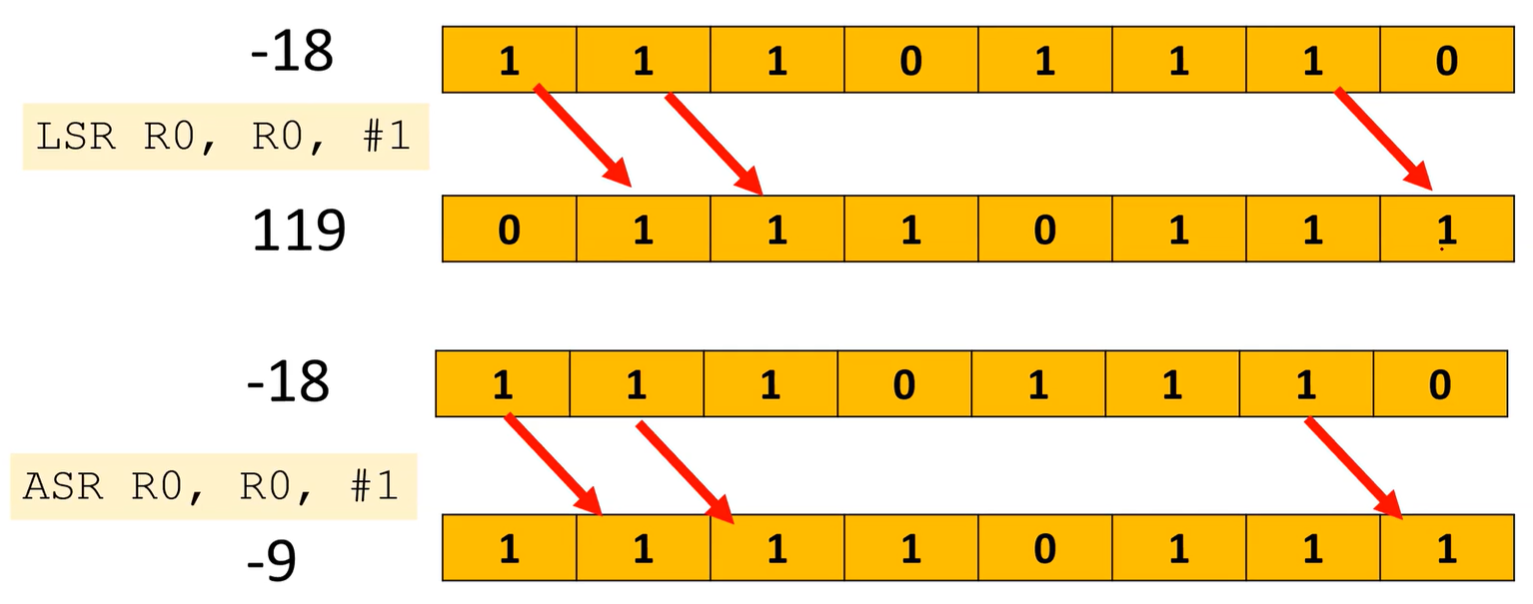
\includegraphics[scale=0.3]{img/lsr_asr.PNG}
\end{center}
Another visual diagram is shown below:
\begin{center}
    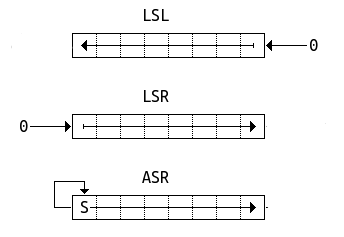
\includegraphics[scale=0.7]{img/lsr_asr_ex.PNG}
\end{center}

\subsection{Assignment Instructions}
Now, we will briefly discuss assignment instructions. 

\subsubsection{Assigning Registers or Immediates}
We can assign registers or intermediates to another register like so:
\begin{center}
    \begin{tabular}{c|c}
        Example (in ARM) & Equivalent to (in C) \\ 
        \hline 
        \code{mov r0, r1} & \code{a = b;} \\ 
        \code{mov r0, \#10} & \code{a = 10;} 
    \end{tabular}
\end{center}
Where ARM registers \code{r0}, \code{r1} are associated with C variables \code{a} and \code{b}, respectively. 

\subsubsection{Move Complement Instruction}
The \code{mvn} instruction moves the one's complement of the operand into the register. You can also think of it as it taking the value of the operand and then performing a bitwise logical NOT operation on the value.  
\begin{center}
    \begin{tabular}{c|c}
        Example (in ARM) & Equivalent to (in C) \\ 
        \hline 
        \code{mvn r0, \#0} & \code{a = -1;} \\ 
        \code{mvn r0, r2} & \code{a = }$\sim$\code{b}
    \end{tabular}
\end{center}
Where ARM registers \code{r0}, \code{r1} are associated with C variables \code{a} and \code{b}, respectively. 

\subsection{Control Transfer}
We will discuss control transfer ARM assembly instructions, which include the following:
\begin{itemize}
    \item Jumping to another instruction. 
    \item Conditional jump.
    \item Jump to a subroutine.  
\end{itemize}

\subsubsection{Conditional Branch}
To perform a conditional branch, we must do the following:
\begin{itemize}
    \item First, set the condition bits (\code{N}, \code{Z}, \code{V}, or \code{C}) in the program status register. 
    \item Then, check on these condition bits to branch conditionally. 
\end{itemize}
Here, the condition bits mean the following:
\begin{itemize}
    \item \code{N}: Negative condition code flag (\code{< 0}). 
    \item \code{Z}: Zero condition code flag (\code{== 0}).
    \item \code{C}: Carry condition code flag.
    \item \code{V}: Overflow condition code flag.
\end{itemize}
% https://www.sciencedirect.com/topics/computer-science/current-program-status-register
These condition codes are defined like so\footnote{You do not need to memorize these.}:
\begin{center}
    \begin{tabular}{c|c|c}
        \textbf{Suffix} & \textbf{Flags}    & \textbf{Meaning} \\ 
        \hline 
        \code{eq}       & \code{Z} set.     & Equal. \\ 
        \code{ne}       & \code{Z} cleared. & Not Equal. \\ 
        \code{le}       & \code{z} set; or \code{n} and \code{v} different. & Less Than or Equal. \\ 
        \code{lt}       & \code{n} and \code{v} different. & Less Than. \\ 
        \code{ge}       & \code{n} and \code{v} same. & Greater Than or Equal. \\ 
        \code{gt}       & \code{z} cleared; or \code{n} and \code{v} same. & Greater Than.
    \end{tabular}
\end{center}

\subsubsection{Comparison Instructions}
To set the condition bits mentioned in the previous subsection, we make use of the \code{cmp} instruction. Essentially, the \code{cmp} instruction compares and sets condition bits. This subtracts a register or an immediate value from a register value and updates the condition code. Unlike \code{sub}, this does not store the results anywhere. 

\bigskip 

Consider the following examples: 
\begin{verbatim}
    cmp     r3, #0   // Set Z flag if r3 == 0, or namely r3 - 0 == 0. 
    cmp     r3, r4   // Set Z flag if r3 == r4, or namely r3 - r4 == 0.
\end{verbatim}

\bigskip 

Obviously, all flags are set as result of this operation, not just \code{Z}. Conditional branches are often preceded by \code{cmp}. 

\subsubsection{Conditional Branches}
ARM has variants of the branch instruction that only goes to the label if a certain condition is \emph{true}. Consider the following table, which contains a subset of all possible conditional branches, where \code{label} is some label:
\begin{center}
    \begin{tabular}{c|c|c}
        \textbf{Instruction} & \textbf{Example} & \textbf{Meaning} \\ 
        \hline 
        \code{b}             & \code{b label}   & Unconditionally goto label. \\ 
        \code{beq}           & \code{beq label} & Branch to Label if equal. \\ 
        \code{bne}           & \code{bne label} & Branch to Label if not equal. \\ 
        \code{ble}           & \code{ble label} & Branch to Label if less than or equal. \\ 
        \code{blt}           & \code{blt label} & Branch to Label if less than. \\ 
        \code{bge}           & \code{bge label} & Branch to Label if greater than or equal. \\ 
        \code{bgt}           & \code{bgt label} & Branch to Label if greater than. 
    \end{tabular}
\end{center}
These conditions are true or false based upon the fields in the program status register. As a final remark, we can use these branches to mimic the behavior of \code{||} and \code{\&\&} when doing comparisons. 

\subsubsection{Various Examples}
Assume \code{X}, \code{Y}, and \code{Z} and integers in registers \code{r0}, \code{r1}, and \code{r2}, respectively. Observe the following C code.
\begin{verbatim}
    if (X == 0) {
        X = Y + Z;
    }
\end{verbatim}
What is the equivalent ARM assembly code? 

\begin{itemize}
    \item Generally, when we want to use labels, we want to negate the condition so we can tell the instruction routine to go to a different place in our code. This makes it significantly easier to manage various conditional statements. 
    \begin{verbatim}
            cmp     r0, #0       // if (X == 0) {
            bne     false_label  //      . 
            add     r0, r1, r2   //      X = Y + Z; 
        false_label:             // }
            ... 
    \end{verbatim}
\end{itemize}

\bigskip 
\bigskip 

Assume \code{X}, \code{Y}, and \code{Z} and integers in registers \code{r0}, \code{r1}, and \code{r2}, respectively. Observe the following C code.
\begin{verbatim}
    if (X == 0) {
        X = Y + Z;
    }
    else {
        X = Y - Z;
    }
\end{verbatim}
What is the equivalent ARM assembly code? 

\begin{itemize}
    \item Same idea as the previous example. 
    \begin{verbatim}
            cmp     r0,#0       // if (X == 0) {
            bne     else_stat   //      .
            add     r0,r1,r2    //      X = Y + Z;
            b       end_if      // }
        else_stat:              // else {
            sub     r0,r1,r2    //      X = Y - Z;
        end_if:                 // }
            ...                 

    \end{verbatim}
\end{itemize}

\bigskip 
\bigskip 

Assume \code{X}, \code{Y}, and \code{Z} and integers in registers \code{r0}, \code{r1}, and \code{r2}, respectively. Observe the following ARM code.
\begin{verbatim}
            mov     r2,#0
        label:
            add     r2,r2,r1
            sub     r0,r0,#1
            cmp     r0,#0
            bne     label 
\end{verbatim}
What is this equvalent to in C?

\begin{itemize}
    \item Annotating this code, we have the following:
    \begin{verbatim}
            mov     r2,#0       // int Z = 0;
        label:                  // while (true) {
            add     r2,r2,r1    //      Z = Z + 1;
            sub     r0,r0,#1    //      X = X - 1;
            cmp     r0,#0       //      if (X == 0) 
            bne     label       //          continue;
                                // } 
    \end{verbatim}
    Or, using a \code{do...while} loop:
    \begin{verbatim}
        int Z = 0;
        do {
            Z = Z + 1;
            X = X - 1;
        } while (X != 0);
    \end{verbatim}
\end{itemize}


% ================================================%
%                NEW SECTION                      %
% ================================================%
\newpage 

\section{32-Bit ARM Assembly (Part 2)}
In this section, we will continue to discuss ARM assembly, but we will talk more about functions and data transfer. 

\subsection{Data Transfer}
We will briefly review data transfer instructions, which interact with memory and involve:
\begin{itemize}
    \item Loading a word from memory into a register. 
    \item Storing the contents of a register into a memory word.
\end{itemize}

\subsubsection{Single Register Data Transfer}
We make use of the following instructions:
\begin{center}
    \begin{tabular}{c|c|c|c}
        \textbf{Load Instruction} & \textbf{Store Instruction} & \textbf{Type} & \textbf{Bits} \\ 
        \hline 
        \code{ldr}                & \code{str}                 & Word          & 32 \\ 
        \code{ldrb}               & \code{strb}                & Byte          & 8  \\ 
        \code{ldrh}               & \code{strh}                & Halfword      & 16 \\ 
        \code{ldrsb}              &                            & Signed Byte Load & 8 \\ 
        \code{ldrsh}              &                            & Signed Halfword Load & 16
    \end{tabular}
\end{center}
A few remarks:
\begin{itemize}
    \item The \code{ldrsh} instruction loads a half-word and sign-extends it to the 32-bits of the register.
    \item The \code{ldrsb} instruction loads a byte and sign-extends it to the 32-bits of the the register. 
    \item The \code{ldrh} instruction loads a half-word and zero-extends the loaded 16-bits to 32-bits.
    \item The \code{ldrb} instruction loads a byte and zero-extends the loaded 8-bits to 32-bits. 
\end{itemize}
The syntax for all of these instructions are as follows:
\begin{verbatim}
    ldr     Rd, <Address> 
    str     Rd, <Address>
\end{verbatim}
Where \code{Rd} is a register.

\subsubsection{Addressing Modes}
There are two ways to specify the address in ARM. We call these \emph{addressing modes}.
\begin{enumerate}
    \item Basic register addressing. 
    \begin{itemize}
        \item Register holds the 32-bit memory address. 
        \item Also known as the base address. 
    \end{itemize}

    \item Base displacement addressing mode. 
    \begin{itemize}
        \item An effective address is calculated using the formula:
        \begin{verbatim}
            Effective Address = Base Address + Offset
        \end{verbatim}
        \item The base address is in a register as before. 
        \item The offset can be specified in different ways. 
    \end{itemize}
\end{enumerate}

\subsubsection{Basic Register Addressing Examples}
\emph{Suppose variable \code{X} is in register \code{r1} and variable \code{Y} is in register \code{r2}. Given the following ARM instruction:}
\begin{verbatim}
    ldr     r2, [r1]
\end{verbatim}
\emph{What is the C equivalent?}

\begin{itemize}
    \item The answer is \code{Y = *X;}.
\end{itemize}

\bigskip 
\bigskip 

\emph{Suppose you have the variable \code{X} in memory at the address contained in the register \code{r1}, and \code{r2} contains the address of \code{Y}. Given the following C code:}
\begin{verbatim}
    Y = &X;
\end{verbatim}
\emph{How would you write this in ARM?}

\begin{itemize}
    \item The answer is \code{str r1, [r2]}. 
\end{itemize}

\bigskip 
\bigskip 

\emph{Suppose you have variable \code{X} in memory at the address contained in \code{r1}, and \code{r2} contains the address of \code{Y}. Given the following C code:}
\begin{verbatim}
    Y = *X;
\end{verbatim}
\emph{How would you write this in ARM?}

\begin{itemize}
    \item The answer is: 
    \begin{verbatim}
        ldr     r10, [r1]
        ldr     r9, [r10]
        str     r9, [r2]
    \end{verbatim}
\end{itemize}

\subsubsection{Base Displacement Addressing Mode}
To specify a memory address to copy from, we need to specify two things.
\begin{itemize}
    \item A register which contains a pointer to memory. 
    \item A numerical offset (in bytes). 
\end{itemize}

The effective memory address is the sum of these two values. For example, given \code{[r0, \#8]}:
\begin{itemize}
    \item This specifies the memory address pointed to by the value in \code{r0}, plus 8 bytes.
    \item \code{r0} is generally called the base address. 
    \item \code{\#8} is generally called the offset. 
\end{itemize}
This is particularly useful for accessing arrays, as we will see. 

\subsubsection{Base Displacement Addressing Examples}
\emph{Given the C code:}
\begin{verbatim}
    X = arr[4];
\end{verbatim}
\emph{Where \code{arr} is an \code{int} array, the base address of \code{arr} is in register \code{r1} and \code{X} is in \code{r2}. What is the assembly equivalent?}

\begin{itemize}
    \item The answer is \code{ldr r2, [r1, 16]}. Recall that an integer is 4 bytes. To access the element at index 4, we need to multiply the size of an integer by the index, so \code{4 * 4 = 16}. 
\end{itemize}

\bigskip 
\bigskip 

\emph{Given the following C code:}
\begin{verbatim}
    g = h + A[8];
\end{verbatim}
Where \code{g} is in \code{r1}, \code{h} is in \code{r2}, and the base address of \code{A} is in \code{r3}. What is the ARM equivalent? 

\begin{itemize}
    \item The answer is:
    \begin{verbatim}
        ldr     r0, [r3, #32]       // r0 = A[4]; (sizeof(int) * 8 = 4 * 8 = 32)
        add     r1, r2, r0          // g = h + r0; 
    \end{verbatim}
\end{itemize}

\subsection{Function Calls}
Here, we will talk about function calls. 

\bigskip 

Recall that a \textbf{caller} is a function that calls another function; a \textbf{callee} is a function that was called. The currently-executing function is a callee, but not a caller.

\subsubsection{Register Usage}
There are 16 registers that we will work with. 
\begin{itemize}
    \item Registers \code{r0} through \code{r3}: Arguments into function. Result(s) from function otherwise corruptible. Additional parameters are passed on stack.
    \item Registers \code{r4} through \code{r11}: Register variables must be preserved. In other words, the value in one of these registers must be the same before and after execution of the function. 
    \begin{itemize}
        \item \code{r9}: Known as the \textbf{stack base} (\code{sb}).
        \item \code{r10}: Known as the \textbf{stack limit} (\code{sl}).
        \item \code{r11}: Known as the \textbf{frame pointer} (\code{fp}).
    \end{itemize}
    \item Register \code{r12}: \textbf{Scratch register}, which is corruptible.
    \item Register \code{r13}: \textbf{Stack pointer} (\code{sp}).
    \item Register \code{r14}: \textbf{Link register} (\code{lr}). This is a register which holds the address to return when a function call completes.\footnote{\code{r14} can be used as a temporary once value stacked.}. 
    \item Register \code{r15}: \textbf{Program counter}. This is a register that indicates where a computer is in its program sequence. Usually, the PC is incremented after fetching an instruction, and holds the memory address of ("points to") the next instruction that would be executed.
\end{itemize}

\subsubsection{Nested Procedures}
Consider the C function:
\begin{verbatim}
    int someFunc(int j, int k) {
        int i, m; 
        i = mult(j, k);
        m = mult(i, i) + j;
        return i + m;
    }
\end{verbatim}
There are a few things to know here.
\begin{itemize}
    \item \code{r0} will always be the first parameter. 
    \item \code{r1} will always be the second parameter. 
    \item When a function returns a value, it will always be in \code{r0}.
\end{itemize}
In the code shown above, \code{r0} is \code{j} as \code{r1} is \code{k}. But, once you call the \code{mult} function, \code{r0} will be the result of the \code{mult} function. However, it's not hard to tell that the original parameter value \code{j} will be overwritten. Thus, you need to save \code{j} to a local variable, or preserved register (\code{r4} through \code{r10}) or you will lose the value. 

\bigskip 

In general, if you have a parameter value (\code{r0} through \code{r3}) that you need to use at some point in the function, save it in a preserved register. 

\subsubsection{Storing Local Variables on the Stack}
When saving things, we need to save it to the stack. Recall that the stack looks something like:
\begin{center}
    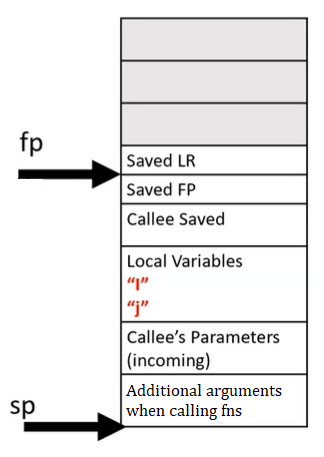
\includegraphics[scale=0.6]{img/i2.PNG}
\end{center}
There are a few things to note here.
\begin{itemize}
    \item If there is a 5th, 6th, or more parameters, it will be put above \code{Saved LR} (above the stack frame). We can load these parameters using:
    \begin{verbatim}
        ldr     Rd, [fp, #4]     // 4 is the location that this 
                                // parameter is stored at. 
    \end{verbatim}
    \item When saving things, we will use the stack frame. The stack frame is bounded by the frame pointer (\code{fp}) and the stack pointer (\code{sp}). The frame pointer is like an anchor; it is the beginning of the stack frame. When you call a function, it generates a new stack frame. 
    \item When you get to a function, you should save the link register (\code{lr}) and the frame pointer (\code{fp}). In particular, we want to change the frame pointer since the frame pointer was pointing to the frame pointer of the previous function (the one that just called said function). 
    \begin{itemize}
        \item You also want to save any potential preserved register (\code{r4} through \code{10}) that you might use. 
        \item Then, you want to save any local variables. 
    \end{itemize}
\end{itemize}
Generally speaking, for a function, we might have ARM code that looks something like this:
\begin{verbatim}
    .equ    FP_OFFSET, 12           // Offset to set fp to base of saved regs.
                                    // (# of Saved Regs - 1) * 4 
    .equ    LOCAL_VAR_SPACE, 8      // Total number of local variable bytes to
                                    // allocate
    .equ    i_OFFSET, -16           // Local var i offset from fp. 
    .equ    j_OFFSET, -20           // Local var j offset from fp. 
    .equ    PARAM_SPACE, 16         // Total number of formal parameter bytes to
                                    // allocate. 
    .equ    PARAM1_OFFSET0, -24     // 1st format param offset from fp. 
    .equ    PARAM2_OFFSET1, -28     // 2nd formal param offset from fp. 

fnEntry: 
    push    {r4-r5, fp, lr}         // Saving just 4 registers. 
    add     fp, sp, #FP_OFFSET      // (# of saved registers - 1) * 4
    sub     sp, sp, #(LOCAL_VAR_SPACE + PARAM_SPACE)
    mov     r4, #10
    str     r4, [fp, #i_OFFSET]
    mov     r4, #20 
    str     r4, [fp, #j_OFFSET]

    ldr     r0, [fp, #i_OFFSET]     // i = i + j;
    ldr     r4, [fp, #j_OFFSET]     // .
    add     r0, r0, r4              // .

    sub     sp, fp, #FP_OFFSET
    pop     {r4, fp, lr}
    bx      lr
\end{verbatim}
A few things to consider. Here, \code{fp} means frame pointer and \code{sp} means stack pointer. We are saving the \code{fp} (frame pointer) of the previous function. The linked register only needs to be saved if it will be altered in this function (say, if we call another function in this function). 
\begin{itemize}
    \item \code{FP\_OFFSET} refers to the number of registers that we are saving. The number of registers that we are saving can be found in the \code{push} instruction. This does not allocate any bytes yet. The formula for this variable is:
    \[(\text{Number of Saved Registers } - 1) \cdot 4\]
    \item \code{LOCAL\_VAR\_SPACE} are the total number of local variable bytes to allocate. Since we have \code{i} and \code{j} (\code{r4} and \code{r5}), we need to allocate 8 bytes.
    \item \code{i\_OFFSET} refers to the local variable \code{i} offset from \code{fp}. \code{j\_OFFSET} refers to the local variable \code{j} offset from \code{fp}. We got these values because:
    \begin{itemize}
        \item \code{Saved LR} is at offset \code{0}.
        \item \code{Saved FP} is at offset \code{-4}.
        \item \code{Callee Saved}\footnote{There is a pretty good explanation on StackOverflow. It reads: \emph{\underline{\textbf{Callee-saved registers}} (AKA non-volatile registers, or call-preserved) are used to hold long-lived values that should be preserved across calls. When the caller makes a procedure call, it can expect that those registers will hold the same value after the callee returns, making it the responsibility of the callee to save them and restore them before returning to the caller. Or to not touch them. By contrast, \underline{\textbf{Caller-saved registers}} (AKA volatile registers, or call-clobbered) are used to hold temporary quantities that need not be preserved across calls. For that reason, it is the caller's responsibility to push these registers onto the stack or copy them somewhere else if it wants to restore this value after a procedure call.}} is at offset \code{-8} and \code{-12} (one for each local variable, if any). For every register you push (using the \code{push} instruction), you should make a note here. 
        \item \code{Local Variable} \code{i} is at offset \code{-16} and \code{j} is at \code{-20}.
    \end{itemize}
    \begin{center}
        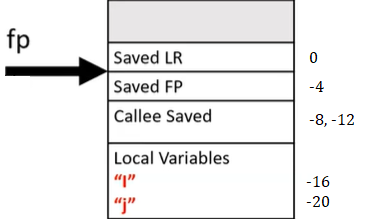
\includegraphics[scale=0.8]{img/i3.PNG}
    \end{center}
    \item \code{PARAM\_SPACE} refers to the number of formal parameter bytes to allocate. This is where you can store the incoming parameters. This refers to \code{r0-r3}. 
    \item \code{PARAM1\_OFFSET0} and \code{PARAM2\_OFFSET1} both follow from the local variable offsets. You use these if you want to save the parameters. 
\end{itemize}

\subsubsection{Accessing Local Variables}
Consider the C function:
\begin{verbatim}
    int num(int a, int b) {
        int c; 
        int d; 
        c = a + b; 
        d = a - b; 
    }
\end{verbatim}
And the preamble:
\begin{verbatim}
    .equ    NUL, 0
    .equ    FP_OFFSET, 4 
    .equ    LOCAL_VAR_SPACE, 8 
    .equ    C_OFFSET, -8 
    .equ    D_OFFSET, -12 
    .equ    PARAM_SPACE, 8 
    .equ    A_OFFSET, -16 
    .equ    B_OFFSET, -20 
\end{verbatim}
Here, we demonstrate how local variables can be accessed: 
\begin{verbatim}
    push    {fp, lr}
    add     fp, sp, #FP_OFFSET 
    sub     sp, sp, #20
    str     r0, [fp, #A_OFFSET]         // c = a + b; 
    str     r1, [fp, #B_OFFSET]         // . 
    ldr     r2, [fp, #A_OFFSET]         // . 
    ldr     r3, [fp, #B_OFFSET]         // . 
    add     r3, r2, r3                  // .
    str     r3, [fp, #C_OFFSET]         // .
    ldr     r2, [fp, #A_OFFSET]         // d = a - b;
    ldr     r3, [fp, #B_OFFSET]         // .
    sub     r3, r2, r3                  // .
    str     r3, [fp, #D_OFFSET]         // .
    nop                                 // .
    mov     r0, r3                      // return d; 
    sub     sp, fp, #FP_OFFSET          // .
    pop     {fp, lr}                    // .
    bx      lr                          // .
\end{verbatim}

\subsection{Recursion}
Now, we will talk about recursion. 

\subsubsection{Recursion in C and ARM: Example}
Consider the factorial function:
\begin{verbatim}
fact:
    push    {r4, r5, fp, lr}
    cmp     r0, #1              // if (n > 1) {
    ble     ret_one             //      .
    mov     r4, r0              //      r4 = r0; 
    sub     r0, r0, #1          //      r0 = r0 - 1;
    bl      fact                //      r0 = r4 * fact(r0);
    mul     r0, r0, r4          //      .
    b       end                 // }
ret_one:                        // else {
    mov     r0, #1              //      r0 = 1;
end:                            // }
    pop     {r4, r5, fp, lr}
    bx      lr                  // return r0; 
main: 
    mov     r0, #1 
    bl      fact 
    mov     r2, r0 
\end{verbatim}
\textbf{Remarks:}
\begin{itemize}
    \item If we didn't save the callee-saved registers, we would have gotten into trouble. This is because we kept clobbering \code{r4}. This was because every call to \code{fact} needs its own value of \code{r4}, or more precisely its own stack frame.
    \item Additionally, if we didn't save the \code{lr} (link register), we would end up with an infinite loop since every call to \code{fact} clobbers the old version of \code{lr}. 
\end{itemize}


% ================================================%
%                NEW SECTION                      %
% ================================================%
\newpage 

\section{Digital Logic}
Now, we will briefly go over digital logic. In particular, we will review combinational logic, timing diagrams, machine code, and more.

\subsection{Logic Gates}
There are a few logic gates to remember.

\subsubsection{AND Gates}
An AND Gate is a basic logic gate which provides \code{1} once all of the inputs to the AND Gate are \code{1}. If any of the input is \code{0}, than its output is \code{0}. It is also referred to as arithmetic multiply operation. It can be represented like so:
\begin{center}
    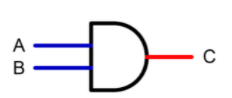
\includegraphics[scale=0.9]{img/l4.PNG}
\end{center}
Here are some common representations of \code{AND}.
\begin{itemize}
    \item $C = A \text{ \& } B$
    \item $C = AB$
    \item $C = A.B$
\end{itemize}
And the truth table is as follows:
\begin{center}
    \begin{tabular}{cc|c}
        \textbf{A} & \textbf{B} & \textbf{C} \\ 
        \hline 
        \code{0} & \code{0} & \code{0} \\ 
        \code{0} & \code{1} & \code{0} \\ 
        \code{1} & \code{0} & \code{0} \\ 
        \code{1} & \code{1} & \code{1}
    \end{tabular}
\end{center}

\subsubsection{OR Gates}
A logical gate which gives \code{0} if only and only when all of the inputs are low state \code{0}. Otherwise, it will give \code{1} as the output. It can be represented like so: 
\begin{center}
    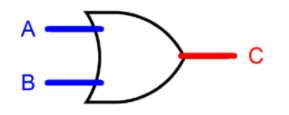
\includegraphics[scale=0.7]{img/l5.PNG}
\end{center}
Some ways to represent \code{OR}: 
\begin{itemize}
    \item $C = A \mid B$
    \item $C = A + B$
\end{itemize}
And the truth table: 
\begin{center}
    \begin{tabular}{cc|c}
        \textbf{A} & \textbf{B} & \textbf{C} \\ 
        \hline 
        \code{0} & \code{0} & \code{0} \\ 
        \code{0} & \code{1} & \code{1} \\ 
        \code{1} & \code{0} & \code{1} \\ 
        \code{1} & \code{1} & \code{1}
    \end{tabular}
\end{center}

\subsubsection{NOT Gates}
A logical NOT gate takes \code{0} or \code{1}, and produces \code{1} and \code{0} respectively as an output. It can be represented like so: 
\begin{center}
    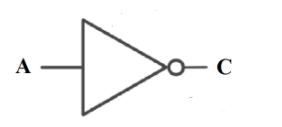
\includegraphics[scale=0.7]{img/l6.PNG}
\end{center}
Some ways to represent \code{NOT}:
\begin{itemize}
    \item $C = \sim A$
    \item $C = A'$
\end{itemize}
And the truth table:
\begin{center}
    \begin{tabular}{c|c}
        \textbf{A} & \textbf{C} \\ 
        \hline 
        \code{0} & \code{1} \\ 
        \code{1} & \code{0}
    \end{tabular}
\end{center}

\subsubsection{NAND Gate}
A logical NAND operates as an AND gate followed by a NOT gate. It can be represented like so (notice the circle at the tip):
\begin{center}
    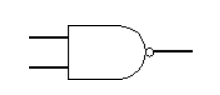
\includegraphics[scale=0.9]{img/l7.PNG}
\end{center}
Some ways to represent \code{NAND}:
\begin{itemize}
    \item $\sim(ab)$
    \item $(ab)'$
\end{itemize}

And the truth table is as follows:
\begin{center}
    \begin{tabular}{cc|c}
        \textbf{A} & \textbf{B} & \textbf{C} \\ 
        \hline 
        \code{0} & \code{0} & \code{1} \\ 
        \code{0} & \code{1} & \code{1} \\ 
        \code{1} & \code{0} & \code{1} \\ 
        \code{1} & \code{1} & \code{0}
    \end{tabular}
\end{center}

\subsubsection{NOR Gate}
A logical NOR operates as an OR gate followed by a NOT gate. It can be represented like so:
\begin{center}
    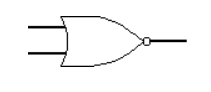
\includegraphics[scale=0.9]{img/l8.PNG}
\end{center}
Some ways to represent \code{NOR}:
\begin{itemize}
    \item $\sim(a|b)$
    \item $\sim(a + b)$
    \item $(a + b)'$
\end{itemize}
And the truth table is as follows:
\begin{center}
    \begin{tabular}{cc|c}
        \textbf{A} & \textbf{B} & \textbf{C} \\ 
        \hline 
        \code{0} & \code{0} & \code{1} \\ 
        \code{0} & \code{1} & \code{0} \\ 
        \code{1} & \code{0} & \code{0} \\ 
        \code{1} & \code{1} & \code{0}
    \end{tabular}
\end{center}

\subsubsection{XOR Gate}
A logical gate which gives \code{1} if \underline{one of two} inputs is \code{1} and \code{0} otherwise. It can be represented like so:
\begin{center}
    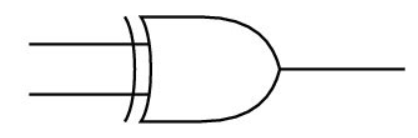
\includegraphics[scale=0.6]{img/l10.PNG}
\end{center}
Some ways to represent \code{XOR}:
\begin{itemize}
    \item $a \wedge b$
    \item $a \oplus b$
\end{itemize}
And the truth table is as follows: 
\begin{center}
    \begin{tabular}{cc|c}
        \textbf{A} & \textbf{B} & \textbf{C} \\ 
        \hline 
        \code{0} & \code{0} & \code{0} \\ 
        \code{0} & \code{1} & \code{1} \\ 
        \code{1} & \code{0} & \code{1} \\ 
        \code{1} & \code{1} & \code{0}
    \end{tabular}
\end{center}

\subsubsection{XNOR Gate}
A logical gate operates as a XOR gate followed by a NOT gate. It can be represented like so:
\begin{center}
    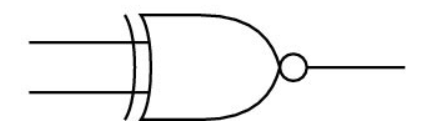
\includegraphics[scale=0.6]{img/l11.PNG}
\end{center}
Some ways to represent \code{XOR}:
\begin{itemize}
    \item $\sim (a \wedge b)$
    \item $(a \oplus b)'$
\end{itemize}
And the truth table is as follows: 
\begin{center}
    \begin{tabular}{cc|c}
        \textbf{A} & \textbf{B} & \textbf{C} \\ 
        \hline 
        \code{0} & \code{0} & \code{1} \\ 
        \code{0} & \code{1} & \code{0} \\ 
        \code{1} & \code{0} & \code{0} \\ 
        \code{1} & \code{1} & \code{1}
    \end{tabular}
\end{center}

\subsubsection{Boolean Laws}
You can use these to help in simplifying boolean expressions. 

\begin{itemize}
    \item Commutative Property 
    \[A + B = B + A\]
    \[AB = BA\]

    \item Associative Property 
    \[A + (B + C) = (A + B) + C\]
    \[A(BC) = (AB)C\]

    \item Distributive Property
    \[A(B + C) = AB + AC\]
    \[A + BC = (A + B)(A + C)\]

    \item DeMorgan's Law
    \[(A + B)' = A'B'\]
    \[(AB)' = A' + B'\]

    \item Other Properties 
    \[A + A'B = A + B\]
    \[A + A' = 1\]
\end{itemize}

\subsection{Timing Diagrams}
\begin{itemize}
    \item In the real world, we represent \code{0} as no voltage and \code{1} as having voltage. 
    \item Gates have a delay. Rather than instantly computing \code{A} and \code{B}, it takes some times for it to compute. 
    \item This can be represented with timing diagrams. 
\end{itemize}
Consider this timing diagram:
\begin{center}
    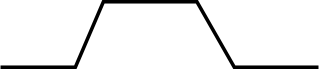
\includegraphics[scale=0.6]{img/timing_diagram.PNG}
\end{center}
\begin{itemize}
    \item The bottom-most line represents \code{0} and the top-most line represents \code{1}.
    \item The line connecting the bottom to the top, known as a rising edge or rise time, is called a positive edge. 
    \item The line connecting the top to the bottom, known as a falling edge or fall time, is called a negative edge.   
\end{itemize}


\subsection{Multiplexer (Mux)}
A simple 2-1 mux, like the one shown below, takes in two bits and produces one bit, depending on the way the third input is set.
\begin{center}
    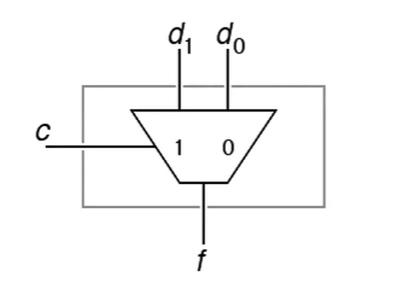
\includegraphics[scale=0.4]{img/mux.PNG}
\end{center}
The truth table for a 2-1 mux is:
\begin{center}
    \begin{tabular}{c|c}
        C & f \\ 
       \hline 
        0 & $d_0$ \\ 
        1 & $d_1$
    \end{tabular}
\end{center}
We can represent this truth table by:
\[f = \begin{cases}
    d_1 & C = 1 \\
    d_0 & C = 0
\end{cases}\]
So:
\begin{itemize}
    \item $f$ should be the value of $d_1$ whenever $C$ is 1. So, $f = c \cdot d_1$.
    \item $f$ should be the value of $d_0$ whenever $C$ is 0. So, $f = \sim C \cdot d_0$. 
\end{itemize}
The expression and its corresponding truth table is:
\[f = C \cdot d_1 \mid \sim C \cdot d_0 \iff f = Cd_1 + C'd_0\]
\begin{center}
    \begin{tabular}{c|c c|c}
        C & $d_0$ & $d_1$ & f \\ 
        \hline 
        0 & 0 & 0 & 0 \\ 
        0 & 0 & 1 & 0 \\ 
        0 & 1 & 0 & 1 \\ 
        0 & 1 & 1 & 1 \\ 
        1 & 0 & 0 & 0 \\ 
        1 & 0 & 1 & 1 \\ 
        1 & 1 & 0 & 0 \\ 
        1 & 1 & 1 & 1
    \end{tabular}
\end{center}


\subsection{Arithmetic Logic Unit (ALU)}
A one-bit ALU looks like this:
\begin{center}
    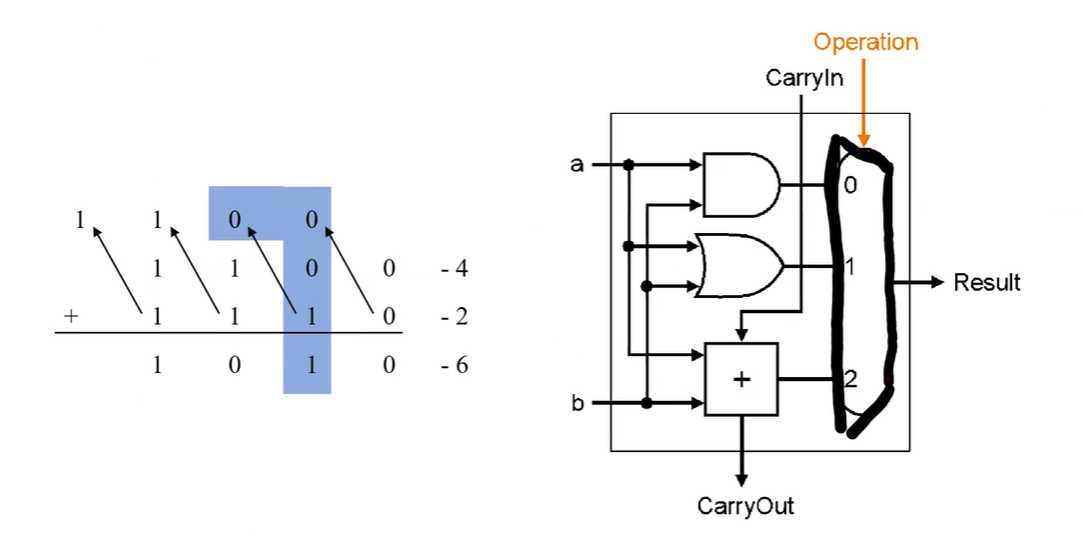
\includegraphics[scale=0.5]{img/1b_alu.PNG}
\end{center}
This ALU can perform \code{ADD}, \code{OR}, and the \code{ADD} operations. 

\subsubsection{32-Bit ALU}
Suppose we wanted a 32-bit ALU. Then, we only need to chain the above one-bit ALU 32 times. That is:
\begin{center}
    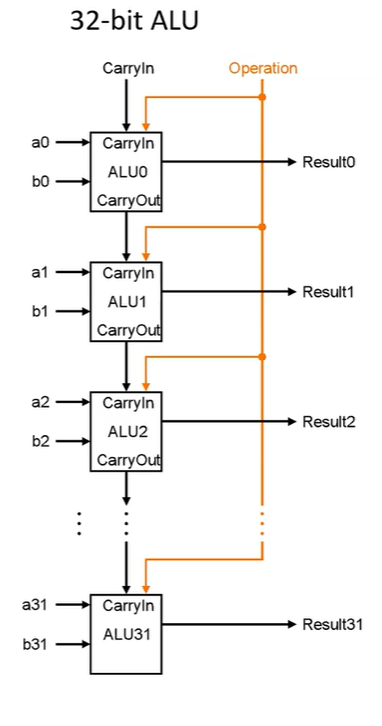
\includegraphics[scale=0.5]{img/32b_alu.PNG}
\end{center}
The carry-out of bit 0 goes to the carry-in of bit 1, the carry-out of bit 1 goes to the carry-in of bit 2, and so on.

\subsubsection{Example Questions}
\emph{We'd like to implement a means of doing $A - B$ (subtraction) but with only minor changes to the above hardware. How can do achieve this?}

\begin{itemize}
    \item Recall that:
    \[A - B = A + (-B)\]
    Our goal is to perform \emph{twos-complement} on $B$ so we can get the desired result. Thus, we need to invert $B$ and then add one to the result. To do this, we need to provide an option to use bitwise \code{NOT B} and then add one. Thus, we need to provide an option to use \code{1} instead of the first carry-in. 
\end{itemize}

\bigskip 
\bigskip 

\emph{Given the full ALU below, what signals accomplish \code{ADD}?}
\begin{center}
    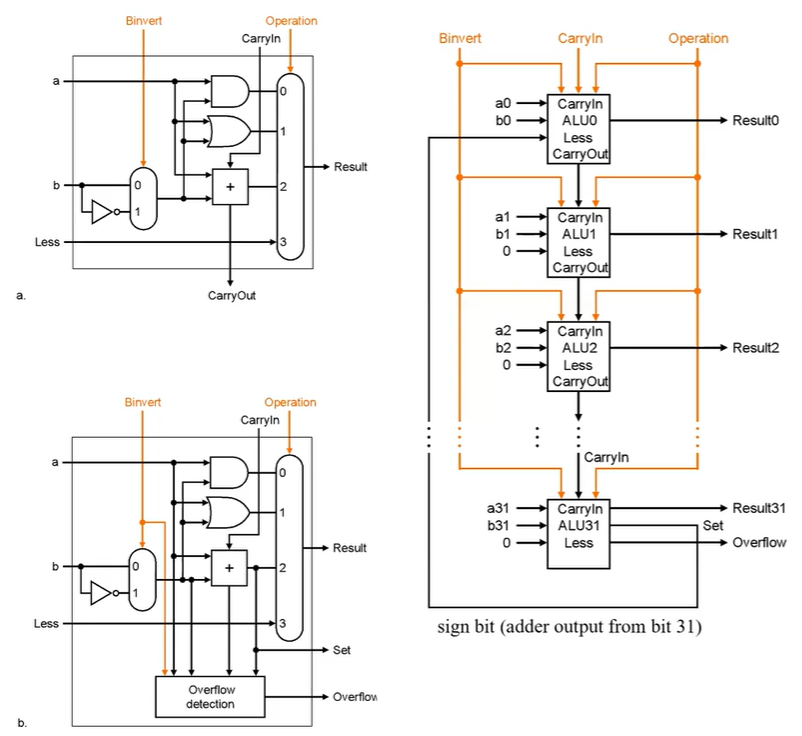
\includegraphics[scale=0.7]{img/full_alu_ex.PNG}
\end{center}

\begin{center}
    \begin{tabular}{c|c|c|c}
          & \code{Binvert} & \code{Carry-In} & \code{Operation} \\ 
        \hline 
        A & 1 & 0 & 0 \\ 
        B & 0 & 1 & 1 \\ 
        C & 1 & 1 & 0 \\ 
        D & 0 & 0 & 1 
    \end{tabular}
\end{center}

\begin{itemize}
    \item The answer is \code{B}. First, we note that the \code{OR} gate is defined by operation \code{1}, so the answers either have to be \code{B} or \code{D}. Now, recall that \code{OR} can be represented by $A + B$. In this sense, it follows that we do \emph{not} want to invert $B$ (which is what answer \code{D} is saying). Thus, the answer is \code{B}.
\end{itemize}

\bigskip 
\bigskip 

\emph{Given the full ALU above, which signals accomplish \code{SUB}?}
\begin{center}
    \begin{tabular}{c|c|c|c}
          & \code{Binvert} & \code{Carry-In} & \code{Operation} \\ 
        \hline 
        A & 1 & 0 & 2 \\ 
        B & 0 & 1 & 2 \\ 
        C & 1 & 1 & 2 \\ 
        D & 0 & 0 & 2 
    \end{tabular}
\end{center}

\begin{itemize}
    \item The answer is \code{C}. Recall that $A - B$ is equivalent to $A + (-B)$. Let's use an example. Suppose we wanted to do $7 - 1$. This is the same as $7 + (-1)$. Of course, we need to take the two's complement of $1$ so we can get $-1$, thus performing $A + (-B)$. In other words:
    \begin{verbatim}
        0001 (1) -> 1110 + 1 = 1111 (-1)
    \end{verbatim}
    Continuing on:
    \begin{verbatim}
            7       0111
        + (-1)    + 1111
        ----------------
            6      10110
    \end{verbatim}
    Discarding the extra bit, we have \code{0110}, which is exactly \code{6}.

    \bigskip 

    Of course, what we just did is exactly the same as inverting $B$ (or simply, $B'$) and then adding 1, and \emph{then} doing $A + (B' + 1)$. Thus, \code{Binvert} is \code{1} and \code{Carry-In} is \code{1}. 
\end{itemize}

\subsection{Sequential Logic}
With combinational logic, we generate a bunch of inputs and generate an output. However, this doesn't actually remember the last thing that we computed. 

\bigskip 

We're going to add a \textbf{state element}, which allows us to save some values so we can use them later. This looks something like the diagram below\footnote{\code{clk} is the clock.}. We will use a clock to distinguish between the different phases of the logic. 
\begin{center}
    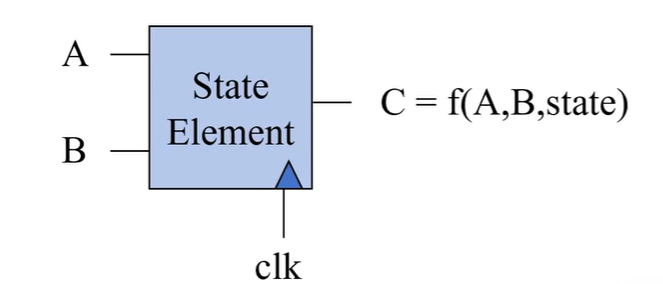
\includegraphics[scale=0.5]{img/state_element.PNG}
\end{center}
One main thing we talked about was the idea of the \textbf{sequential network}. A sequential network looks something like: 
\begin{center}
    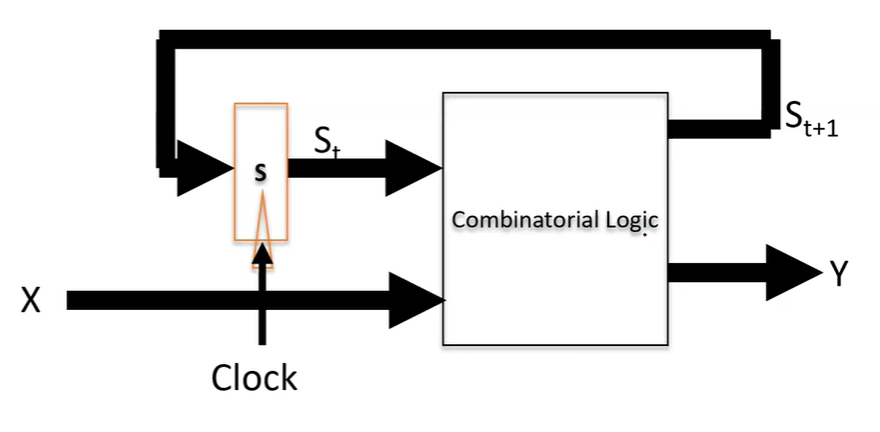
\includegraphics[scale=0.3]{img/sequential_network.PNG}
\end{center}

It has combinational logic (which computes something and then saves it) and state elements (which will save the state).

\bigskip 

For every clock cycle:
\begin{itemize}
    \item Use combinational logic to compute something given an input $X$. 
    \item Output that result. This is simply:
    \[Y = f(S_t, X)\]
    \item Save the result into $S_{t + 1}$. This is:
    \[S_{t + 1} = g(S_t, X)\]
\end{itemize}

\subsubsection{Set/Reset Latch (S-R Latch)}
The SR latch has two inputs \underline{S}et and \underline{R}eset, and another two inputs $Q$ and $\overline{Q}$ (the inverse of $Q$) and can be constructed from a pair of \code{NOR} gates. It looks like:
\begin{center}
    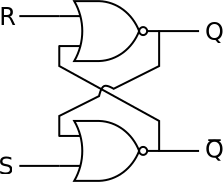
\includegraphics[scale=0.5]{img/SR_latch.png}
\end{center}

\subsubsection{Example Questions}
\emph{Consider the following diagram:}
\begin{center}
    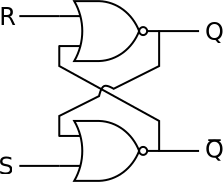
\includegraphics[scale=0.5]{img/SR_latch.png}
\end{center}
\emph{Recall that $\overline{Q} = Q' = \sim Q$. Suppose $S = 1$ and $R = 0$. What will $Q$ be?}
\begin{center}
    \begin{tabular}{c|c}
        \textbf{Selection} & $\mathbf{Q}$ \\ 
        \hline 
        A & 0 \\ 
        B & 1 \\ 
        C & $Q$ from before. \\ 
        D & $Q'$ from before. \\ 
        E & None of the above.
    \end{tabular}
\end{center}

\begin{itemize}
    \item The answer is \code{B}. For $S(\text{Set})$, we are given \code{1}. Although we don't know the value of the other input, we know that $(1 + b)'$ (or $1 \text{ NOR } b$) will always be \code{0}. With this in mind, we know that the gate associated with $S(\text{Set})$ will output \code{0}. Thus, we now know that $R(\text{Reset})$ will have inputs \code{0} (given) and \code{0} (which we got from $S(\text{Set})$). Since $(0 + 0)'$ (or $0 \text{ NOR 0}$) is \code{1}, we know that $Q$ will be \code{1}. 
\end{itemize}

\bigskip 
\bigskip 

\emph{Using the diagram and answer choices from the previous question, and suppose $S = R = 0$. What will $Q$ be?}

\begin{itemize}
    \item Let's make a few assumptions.
    \begin{itemize}
        \item Suppose $Q = 1$. Then, $R(\text{Reset})$ will output \code{1}. This means that the bottom gates will be given two inputs: \code{0} (given) and \code{1} (from the top gate). We know that $(0 + 1)'$ ($0 \text{ NOR } 1$) will produce \code{0}, so the bottom gate will output \code{0}. Then, going to the top gate, we have inputs \code{0} (given) and \code{0} (from the bottom gate), which gives us \code{1}. 
        \item Suppose $Q = 0$. Then, $R(\text{Reset})$ will output \code{0}. This means that the bottom gates will be given inputs \code{0} (given) and \code{0} (from top gate). Since $0 \text{ NOR } 0$ is \code{1}, it follows that the bottom gate will output \code{1}. Then, going back to the top gate, we have inputs \code{0} (given) and \code{1} (from bottom gate), which gives us \code{0}. 
    \end{itemize}
    In both cases, we have showed that for a given input $Q$, we will always get the same $Q$. Thus, the answer is \code{C}. 
\end{itemize}

\subsubsection{Issues with the Set/Reset Latch}
What if $S = R = 1$? Then, $Q = \overline{Q} = 0$, which violates the idea that $\overline{Q}$ is the inverse of $Q$.
\begin{center}
    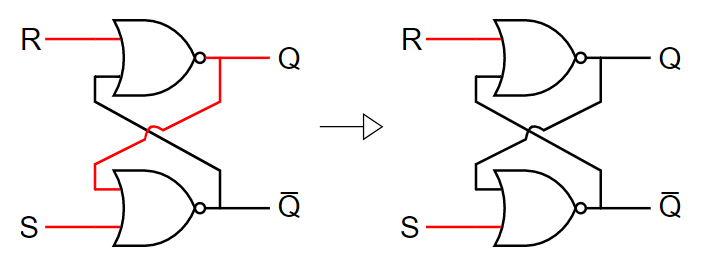
\includegraphics[scale=0.5]{img/sr_bad_1.PNG}
\end{center}

This also creates another issue. That is, once we set $S = R = 0$ at the same time, both \code{NOR} gates will try to output a \code{1} at the same time, which will cause both \code{NOR} gates to output \code{0}s. In this sense, the S-R latch will keep oscillating back and forth until one \code{NOR} gate ``wins'' due to physical differences. This leaves the S-R latch in an unknown issue. 
\begin{center}
    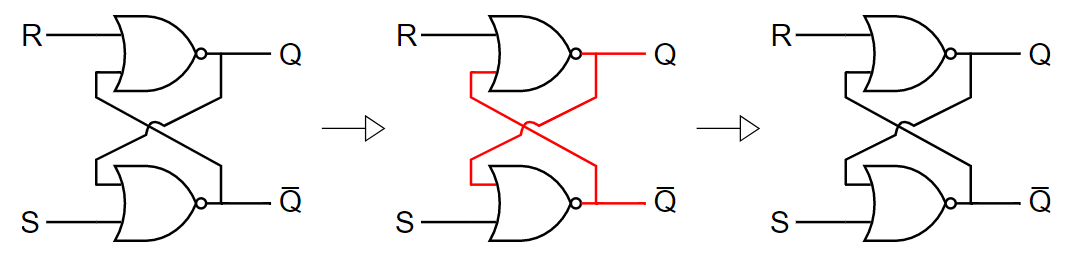
\includegraphics[scale=0.5]{img/sr_bad_2.PNG}
\end{center}

\subsubsection{Clock Signals}
One way to resolve this issue is through the idea of a \underline{clock}. In a computer, a clock is a thing that provides a synchronization point so that as a computer is changing from one state to another, it is done based on a \emph{clock cycle}. So, really, a clock is just a periodic signal that oscillates. 
\begin{center}
    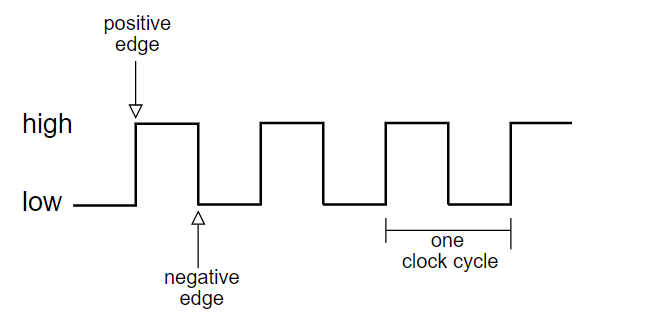
\includegraphics[scale=0.5]{img/clock.PNG}
\end{center}
The clock cycle time, also known as the \emph{period}, is the time between positive edges of a clock signal. This is defined by:
\[\text{Frequency} = \frac{1}{\text{Period}}\]

\subsubsection{Back to the S-R Latch}
We now need to synchronize our S-R latch. To do this, we'll add a clock. 
\begin{center}
    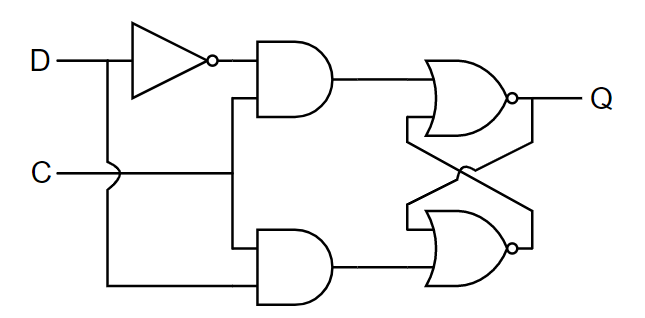
\includegraphics[scale=0.5]{img/new_sr.PNG}
\end{center}
Where our inputs are:
\begin{itemize}
    \item $D$, the data. 
    \item $C$, the clock. 
\end{itemize}
Here, we have a D-latch. When $C$ is low, both inputs to our S-R latch are low\footnote{Low means \code{0}; high means \code{1}.}, meaning the latch holds its state no matter what is happening to $D$. When $C$ is high, $Q$ gets set to $D$'s current state. 

\bigskip 

To summarize, we have:
\begin{center}
    \begin{tabular}{c|c|c}
        \code{C} & \code{D} & Next State of \code{Q} \\ 
        \hline 
        0 & X & No Change \\ 
        1 & 0 & \code{Q = 0}; Reset State \\ 
        1 & 1 & \code{Q = 1}; Set State 
    \end{tabular}
\end{center}

\begin{itemize}
    \item When $C = 1$, the latch is ``transparent''; $Q = D$. 
    \item When $C = 0$, $Q$ is latched to the last value of $D$. 
\end{itemize}

TODO

\subsection{Machine Code}
We want to gain an understanding of machine code so we can bridge the gap between what we know and what the machine knows.

\subsubsection{Data Processing Instruction}
To represent data processing instructions in machine code, we make use of this format:
\begin{center}
    \resizebox{\columnwidth}{!}{
        \begin{tabular}{|c|c|c|c|c|c|c|c|c|}
            \hline 
            \code{31 30 29 28} & \code{27} & \code{26} & \code{25} & \code{24 23 22 21} & \code{20} & \code{19 18 17 16} & \code{15 14 13 12} & \code{11 10 9 8 7 6 5 4 3 2 1 0} \\ 
            \hline 
            \code{Cond} & \code{0} & \code{0} & \code{I} & \code{Opcode} & \code{S} & \code{Rn} & \code{Rd} & \code{Operand 2} \\ 
            \hline 
        \end{tabular}
    }
\end{center}
Where:
\begin{itemize}
    \item \code{Cond} - Does this instruction execute conditionally? In this class, this will always be \code{1110}.\footnote{In CSE 30, we don't care about this.}
    \item \code{I} - Is operand 2 a register or immediate? 
    \begin{itemize}
        \item \code{0} if operand 2 is a register. 
        \item \code{1} if operand 2 is an immediate. 
    \end{itemize}
    \item \code{Opcode} - What data processing instruction are we using? 
    \begin{center}
        \begin{tabular}{c|c|c}
            \textbf{Opcode} & \textbf{Operation} & \textbf{Action} \\ 
            \hline 
            \code{0000} & \code{AND} & \code{Op1 AND Op2} \\ 
            \code{0001} & \code{EOR} & \code{Op1 EOR Op2} \\ 
            \code{0010} & \code{SUB} & \code{Op1 - Op2} \\ 
            \code{0011} & \code{RSB} & \code{Op2 - Op1} \\ 
            \code{0100} & \code{ADD} & \code{Op1 + Op2} \\ 
            \code{0101} & \code{ADC} & \code{Op1 + Op2 + Carry} \\ 
            \code{0110} & \code{SBC} & \code{Op1 - Op2 + Carry - 1} \\ 
            \code{0111} & \code{RSC} & \code{Op2 - Op1 + Carry - 1} \\ 
            \code{1000} & \code{TST} & Set Condition Code on \code{Op1 AND Op2} \\ 
            \code{1001} & \code{TEQ} & Set Condition Code on \code{Op1 EOR Op2} \\ 
            \code{1010} & \code{CMP} & Set Condition Code on \code{Op1 - Op2} \\ 
            \code{1011} & \code{CMN} & Set Condition Code on \code{Op1 + Op2} \\
            \code{1100} & \code{ORR} & \code{Op1 OR Op2} \\ 
            \code{1101} & \code{MOV} & \code{Op2} \\ 
            \code{1110} & \code{BIC} & \code{Op1 AND NOT Op2} \\ 
            \code{1111} & \code{MVN} & \code{NOT Op2}  
        \end{tabular}
    \end{center}
    \item \code{S} - Whether this will set condition codes. In CSE 30, only \code{cmp} and \code{tst} set condition codes. 
    \begin{itemize}
        \item \code{0} if we are not altering condition codes. 
        \item \code{1} if we are setting condition codes. 
    \end{itemize}
    \item \code{Rn} - The first operand register. 
    \item \code{Rd} - The destination register. 
    \item \code{Operand 2} - This depends. 
    \begin{itemize}
        \item If we are working with a register (\code{I} is \code{0}), then\footnote{In CSE 30, the shift will be 0.}:
        \begin{center}
            \begin{tabular}{|c|c|}
                \hline 
                \code{11 10 9 8 7 6 5 4} & \code{3 2 1 0} \\ 
                \hline 
                \code{00000000} & \code{Operand 2} \\ 
                \hline 
            \end{tabular}
        \end{center}

        \item If we are working with an immediate (\code{I} is \code{1}), then:
        \begin{center}
            \begin{tabular}{|c|c|}
                \hline 
                \code{11 10 9 8} & \code{7 6 5 4 3 2 1 0} \\ 
                \hline 
                \code{Rotate} & \code{Imm} \\ 
                \hline 
            \end{tabular}
        \end{center}
        Where \code{Rotate} is the shift applied to \code{Imm} and \code{Imm} is an unsigned 8-bit immediate value. In this class, assume that \code{Rotate} is \code{0000}. That is:
        \begin{center}
            \begin{tabular}{|c|c|}
                \hline 
                \code{11 10 9 8} & \code{7 6 5 4 3 2 1 0} \\ 
                \hline 
                \code{0000} & \code{Imm} \\ 
                \hline 
            \end{tabular}
        \end{center}
    \end{itemize}
\end{itemize}

As an example, suppose we wanted to find the corresponding machine code for \code{add r0, r0, r1}. Then, we know that:
\begin{itemize}
    \item \code{Cond} is \code{1110}.
    \item \code{I} is \code{0} (we're working with a register). 
    \item \code{OpCode} is \code{0100}. 
    \item \code{S} is \code{0} (we aren't using \code{cmp} or \code{tst}). 
    \item \code{Rn} (which is \code{r0}, or the middle register) is \code{0000}. 
    \item \code{Rd} (which is \code{r0}, or the left-most register) is \code{0000}. 
    \item \code{Operand 2} is \code{00000000 0001}. 
\end{itemize}
So, in binary, the corresponding machine code is:
\begin{verbatim}
    1110 000 0100 0 0000 0000 00000000 0001
    0xe08000
\end{verbatim}

\subsubsection{Single Data Transfer Instruction}
To represent single data transfer in machine code, we make use of this format: 

\begin{center}
    \resizebox{\columnwidth}{!}{
        \begin{tabular}{|c|c|c|c|c|c|c|c|c|c|c|} 
            \hline 
            \code{31 30 29 28} & \code{27 26} & \code{25} & \code{24} & \code{23} & \code{22} & \code{21} & \code{20} & \code{19 18 17 16} & \code{15 14 13 12} & \code{11 10 9 8 7 6 5 4 3 2 1 0} \\ 
            \hline 
            \code{Cond} & \code{01} & \code{I} & \code{P} & \code{U} & \code{B} & \code{W} & \code{L} & \code{Rn} & \code{Rd} & \code{Offset} \\ 
            \hline 
        \end{tabular}
    }
\end{center}
Where:
\begin{itemize}
    \item \code{Cond} - The condition field. 
    \begin{center}
        \begin{tabular}{c|c|c|c}
            \code{cond} & \textbf{Mnemonic} & \textbf{Name} & \textbf{CondEx} \\ 
            \hline 
            \code{0000} & \code{EQ} & Equal & $Z$ \\ 
            \code{0001} & \code{NE} & Not Equal & $\overline{Z}$ \\ 
            \code{0010} & \code{CS/HS} & Carry Set/Unsigned Higher or Same & $C$ \\ 
            \code{0011} & \code{CC/LO} & Carry Clear/Unsigned Lower & $\overline{C}$ \\ 
            \code{0100} & \code{MI} & Minus/Negative & $N$ \\ 
            \code{0101} & \code{PL} & Plus/Positive or Zero & $\overline{N}$ \\ 
            \code{0110} & \code{VS} & Overflow/Overflow Set & $V$ \\ 
            \code{0111} & \code{VC} & No Overflow/Overflow Clear & $\overline{V}$ \\ 
            \code{1000} & \code{HI} & Unsigned Higher & $\overline{Z}C$ \\ 
            \code{1001} & \code{LS} & Unsigned Lower or Same & $Z$ or $\overline{C}$ \\ 
            \code{1010} & \code{GE} & Signed Greater Than or Equal & $\overline{N \oplus V}$ \\ 
            \code{1011} & \code{LT} & Signed Less Than & $N \oplus V$ \\ 
            \code{1100} & \code{GT} & Signed Greater Than & $\overline{Z}(\overline{N \oplus V})$ \\ 
            \code{1101} & \code{LE} & Signed Less Than or Equal & $Z$ or $N \oplus V$ \\ 
            \code{1110} & \code{AL} & Always/Unconditional & Ignored
        \end{tabular}
    \end{center}
    \item \code{I} - Whether the offset is is a immediate value (\code{0}) or a register (\code{1}).
    \item \code{P U B W L} - Various bits.
    \begin{center}
        \begin{tabular}{|c|c|c|}
            \hline 
            Bit & \code{T} & \code{U} \\ 
            \hline  
            0 & Immediate Offset in \code{Offset} & Subtract Offset from Base \\ 
            1 & Register Offset in \code{Offset} & Add Offset to Base. \\ 
            \hline 
        \end{tabular}

        \begin{tabular}{|c|c|c|}
            \hline 
            \code{P} & \code{W} & Index Mode \\ 
            \hline  
            0 & 0 & Post-Index \\ 
            0 & 1 & Not Supported \\ 
            1 & 0 & Offset \\ 
            1 & 1 & Pre-Index \\ 
            \hline 
        \end{tabular}
        
        \begin{tabular}{|c|c|c|}
            \hline 
            \code{L} & \code{B} & Instruction \\ 
            \hline 
            0 & 0 & \code{STR} \\ 
            0 & 1 & \code{STRB} \\ 
            1 & 0 & \code{LDR} \\ 
            1 & 1 & \code{LDRB} \\ 
            \hline 
        \end{tabular}

        \begin{tabular}{|c|c|c|c|}
            \hline 
            Mode & ARM Assembly & Address & Base Register \\ 
            \hline 
            Offset & \code{LDR R0, [R1, R2]} & \code{R1 + R2} & Unchanged \\ 
            Pre-Index & \code{LDR R0, [R1, R2]!} & \code{R1 + R2} & \code{R1 = R1 + R2} \\
            Post-Index & \code{LDR R0, [R1], R2} & \code{R1} & \code{R1 = R1 + R2} \\ 
            \hline 
        \end{tabular}
    \end{center}

    \item \code{Rn} - The base operand register. 
    \item \code{Rd} - The source/destination register. 
    \item \code{Offset} - This depends. 
    \begin{itemize}
        \item If we are working with a register (\code{I} is \code{0}), then:
        \begin{center}
            \begin{tabular}{|c|}
                \hline 
                \code{11 10 9 8 7 6 5 4 3 2 1 0} \\ 
                \hline 
                The Immediate Offset \\ 
                \hline 
            \end{tabular}
        \end{center}

        \item If we are working with an immediate (\code{I} is \code{1}), then:
        \begin{center}
            \begin{tabular}{|c|c|}
                \hline 
                \code{11 10 9 8 7 6 5 4} & \code{3 2 1 0} \\ 
                \hline 
                Shift & \code{Rm} \\ 
                \hline 
            \end{tabular}
        \end{center}
        Where \code{Rm} is the offset register.
    \end{itemize}
\end{itemize}

As an example, suppose we are given the following:
\begin{verbatim}
    1110 01 1 1 1 0 0 1 0010 0100 0000 0000 0011
\end{verbatim}
\begin{itemize}
    \item We know that:
    \begin{itemize}
        \item \code{I} is \code{1}, so we're working with a register. 
        \item \code{P} is \code{1} and \code{W} is \code{0}, so we're working with an offset.
        \item \code{U} is \code{1}, so we're adding the offset to the base. 
        \item \code{L} is \code{1} and \code{B} is \code{0}, so we're working with \code{LDR}. 
        \item \code{Rn} is \code{0010}, so the base operand register is \code{r2}. 
        \item \code{Rd} is \code{0100}, so the source/destination register is \code{r4}. 
        \item Since \code{I} is \code{1}, we know that \code{Rm} is \code{0011}, so the offset register is \code{r3}. 
    \end{itemize}
    So, the answer is:
    \begin{verbatim}
        ldr     r4, [r2, r3]
    \end{verbatim}
\end{itemize}

\subsubsection{Branch Instruction}
To represent branch instructions in machine code, we make use of this format: 

\begin{center}
    \resizebox{\columnwidth}{!}{
        \begin{tabular}{|c|c|c|c|} 
            \hline 
            \code{31 30 29 28} & \code{27 26 25} & \code{24} & \code{23 22 21 20 19 18 17 16 15 14 13 12 11 10 9 8 7 6 5 4 3 2 1 0} \\ 
            \hline 
            \code{Cond} & \code{101} & \code{L} & \code{Offset} \\ 
            \hline 
        \end{tabular}
    }
\end{center}

Where: 
\begin{itemize}
    \item \code{Cond} - The condition field. Refer to the table in the previous page. 
    \item \code{L} - The link bit. 
    \begin{itemize}
        \item If this is just a branch, this is \code{0}.
        \item If this is a branch with link, this is \code{1}. 
    \end{itemize}
    The branch instructions contain a signed twos-complement 24-bit offset. This is shifted left two bits, sign-extended to 32-bits, and added to the \code{PC}. The branch offset must take account of the pre-fetch operation, which causes the PC to be 2 words\footnote{1 word is 4 bytes.} (8 bytes) ahead of the current instruction. 
\end{itemize}

For example, suppose we have the following ARM code:
\begin{verbatim}
8004:       cmp     r2, r3 
8008:       blt     label           // ?
8012:       add     r0, r0, r1 
8016:       sub     r0, r0, r3 
8020:       str     r0, [r4]
8024:       b       end 
8028:   label:                      // ?
8032:       add     r0, r0, r2  
\end{verbatim}
What should the offset (in decimal) be for the bit instruction?

\begin{itemize}
    \item We are interested in the branch instruction and the associated label. We know that the branch is at \code{8008}, which is the \code{PC}. But, the program counter must be 2 words ahead of the current instruction, so \code{PC} is at \code{8016}. The target label is at \code{8028}, so $8028 - 8016 = 12$ bytes. But, since 12 bytes is 3 words, the answer is 3. 
\end{itemize}

\end{document}